\documentclass[10pt,conference]{IEEEtran}
%\IEEEoverridecommandlockouts
% The preceding line is only needed to identify funding in the first footnote. If that is unneeded, please comment it out.
\usepackage{cite}
\usepackage{amssymb,amsfonts}
%amsmath,
\usepackage{mathtools}

\usepackage{algorithmic}
\usepackage{graphicx}
\usepackage{textcomp}
\usepackage{xcolor}
\usepackage{bussproofs}

\usepackage{pgf}
\usepackage{tikz}
\usepackage[utf8]{inputenc}
\usetikzlibrary{arrows,automata}
\usetikzlibrary{positioning}

\usepackage{etoolbox}
\usepackage{holtexbasic,url,amsmath,environ}
\renewcommand{\HOLTokenTurnstile}{\ensuremath{\vdash\!\!}}
\renewcommand{\HOLinline}[1]{\ensuremath{#1}}
\renewcommand{\HOLKeyword}[1]{\mathsf{#1}}
\renewcommand{\HOLConst}[1]{{\textsf{\upshape #1}}}
\renewcommand{\HOLTyOp}[1]{\textsf{\itshape #1}}
\renewcommand{\HOLSymConst}[1]{\HOLConst{#1}}
\renewcommand{\HOLTokenBar}{\ensuremath{\mathtt{|}}}

\newtheorem{theorem}{Theorem}
\newtheorem{corollary}{Corollary}
\newtheorem{definition}{Definition}
\newtheorem{remark}{Remark}
\newtheorem{example}{Example}
\newtheorem{conjecture}{Desideratum}
\ifdef{\dpspecial}{
%% tmp by Dirk
\newcommand{\HOLtm}[1]{\texttt{#1}}
\newcommand{\HOLty}[1]{\texttt{#1}}
\newcommand{\HOLthm}[2][]{\texttt{#2}}
\newcommand{\n}{\\n}
}{}
\NewEnviron{holthmenv}{\[\begin{array}[t]{l}\BODY\end{array}\]\ignorespacesafterend}
\newcommand{\TODO}[1]{{\bf TODO:} #1}

\def\BibTeX{{\rm B\kern-.05em{\sc i\kern-.025em b}\kern-.08em
    T\kern-.1667em\lower.7ex\hbox{E}\kern-.125emX}}
\begin{document}

\title{Modular Synthesis of Verified Verifiers of Computation with STV Algorithms}
%*\\
%{\footnotesize \textsuperscript{*}Note: Sub-titles are not captured in Xplore and
%should not be used}
%\thanks{Identify applicable funding agency here. If none, delete this.}


\author{\IEEEauthorblockN{Milad K. Ghale}
\IEEEauthorblockA{\textit{The Australian National University} \\
%\textit{name of organization (of Aff.)}\\
Canberra, Australia \\
milad.ketabghale@anu.edu.au}
\and
\IEEEauthorblockN{Dirk Pattinson}
\IEEEauthorblockA{\textit{The Australian National University} \\
%\textit{name of organization (of Aff.)}\\
Canberra, Australia \\
dirk.pattinson@anu.edu.au}
\and
\IEEEauthorblockN{Michael Norrish}
\IEEEauthorblockA{\textit{Data61, CSIRO, and ANU} \\
%\textit{Data61, CSIRO, and ANU}\\
Canberra, Australia \\
Michael.Norrish@data61.csiro.au}
%\and
%\IEEEauthorblockN{4\textsuperscript{th} Given Name Surname}
%\IEEEauthorblockA{\textit{dept. name of organization (of Aff.)} \\
%\textit{name of organization (of Aff.)}\\
%City, Country \\
%email address}
%\and
%\IEEEauthorblockN{5\textsuperscript{th} Given Name Surname}
%\IEEEauthorblockA{\textit{dept. name of organization (of Aff.)} \\
%\textit{name of organization (of Aff.)}\\
%City, Country \\
%email address}
%\and
%\IEEEauthorblockN{6\textsuperscript{th} Given Name Surname}
%\IEEEauthorblockA{\textit{dept. name of organization (of Aff.)} \\
%\textit{name of organization (of Aff.)}\\
%City, Country \\
%email address}
}

\maketitle
\begin{abstract}
Single transferable vote (STV) is a family of preferential voting systems, different instances of which are used in binding elections throughout the world. We give a formal specification of this family, from which we derive fully verified tools that verify the computation for various instances of STV vote counting. These tools validate 
%the probably correct execution of a run of a 
 an execution of an STV vote counting algorithm, based on a transcript of the count.

Our framework distils the similarities and differences of various instances of STV and gives a uniform and modular way of synthesising verifiers for its various instances, and provides the flexibility and ease for adapting and extending it to a variety of STV schemes. We minimise the trusted base in correctness of the tools produced by using the HOL4 and CakeML as the technical basis. We first formally specify and verify the tools in HOL4 and then obtain the machine executable versions for the tools by relying on the verified proof translator and the compiler of CakeML. Moreover, proofs that we establish in HOL4 and CakeML are almost completely automated so that new verified instances of STV can be created with no (or minimal) extra proof. Finally, our experimental results with executable code demonstrate feasibility of deploying the framework for verifying real size elections having an STV counting algorithm.
\end{abstract}

\begin{IEEEkeywords}
Framework, Modularity, Single Transferable Voting, Algorithms, Veriable Computation, Proof Engineering, Code Synthesis, Elections, Trustworthiness, Transparency 
\end{IEEEkeywords}
\section{Introduction}\label{sec:intro}
%\setlength{\abovedisplayskip}{0.5em}
%\setlength{\belowdisplayskip}{0.5em}
Single transferable vote (STV)\cite{DFar} is a preferential voting scheme used in various jurisdictions around the world, including Ireland, Malta, India, Pakistan, Australia, New Zealand and some municipalities of the United States, typically for multi-seat constituencies.  A ballot is a preference-ordered list of candidates, typically obtained specifying a numerical preference for each candidate appearing on the ballot paper.
% as illustrated in Figure
%\footnote{DP: remove figure and explain textually if low on space}
%\ref{fig:ballot}. 


%\begin{figure}\label{fig:ballot}
%\begin{center}
%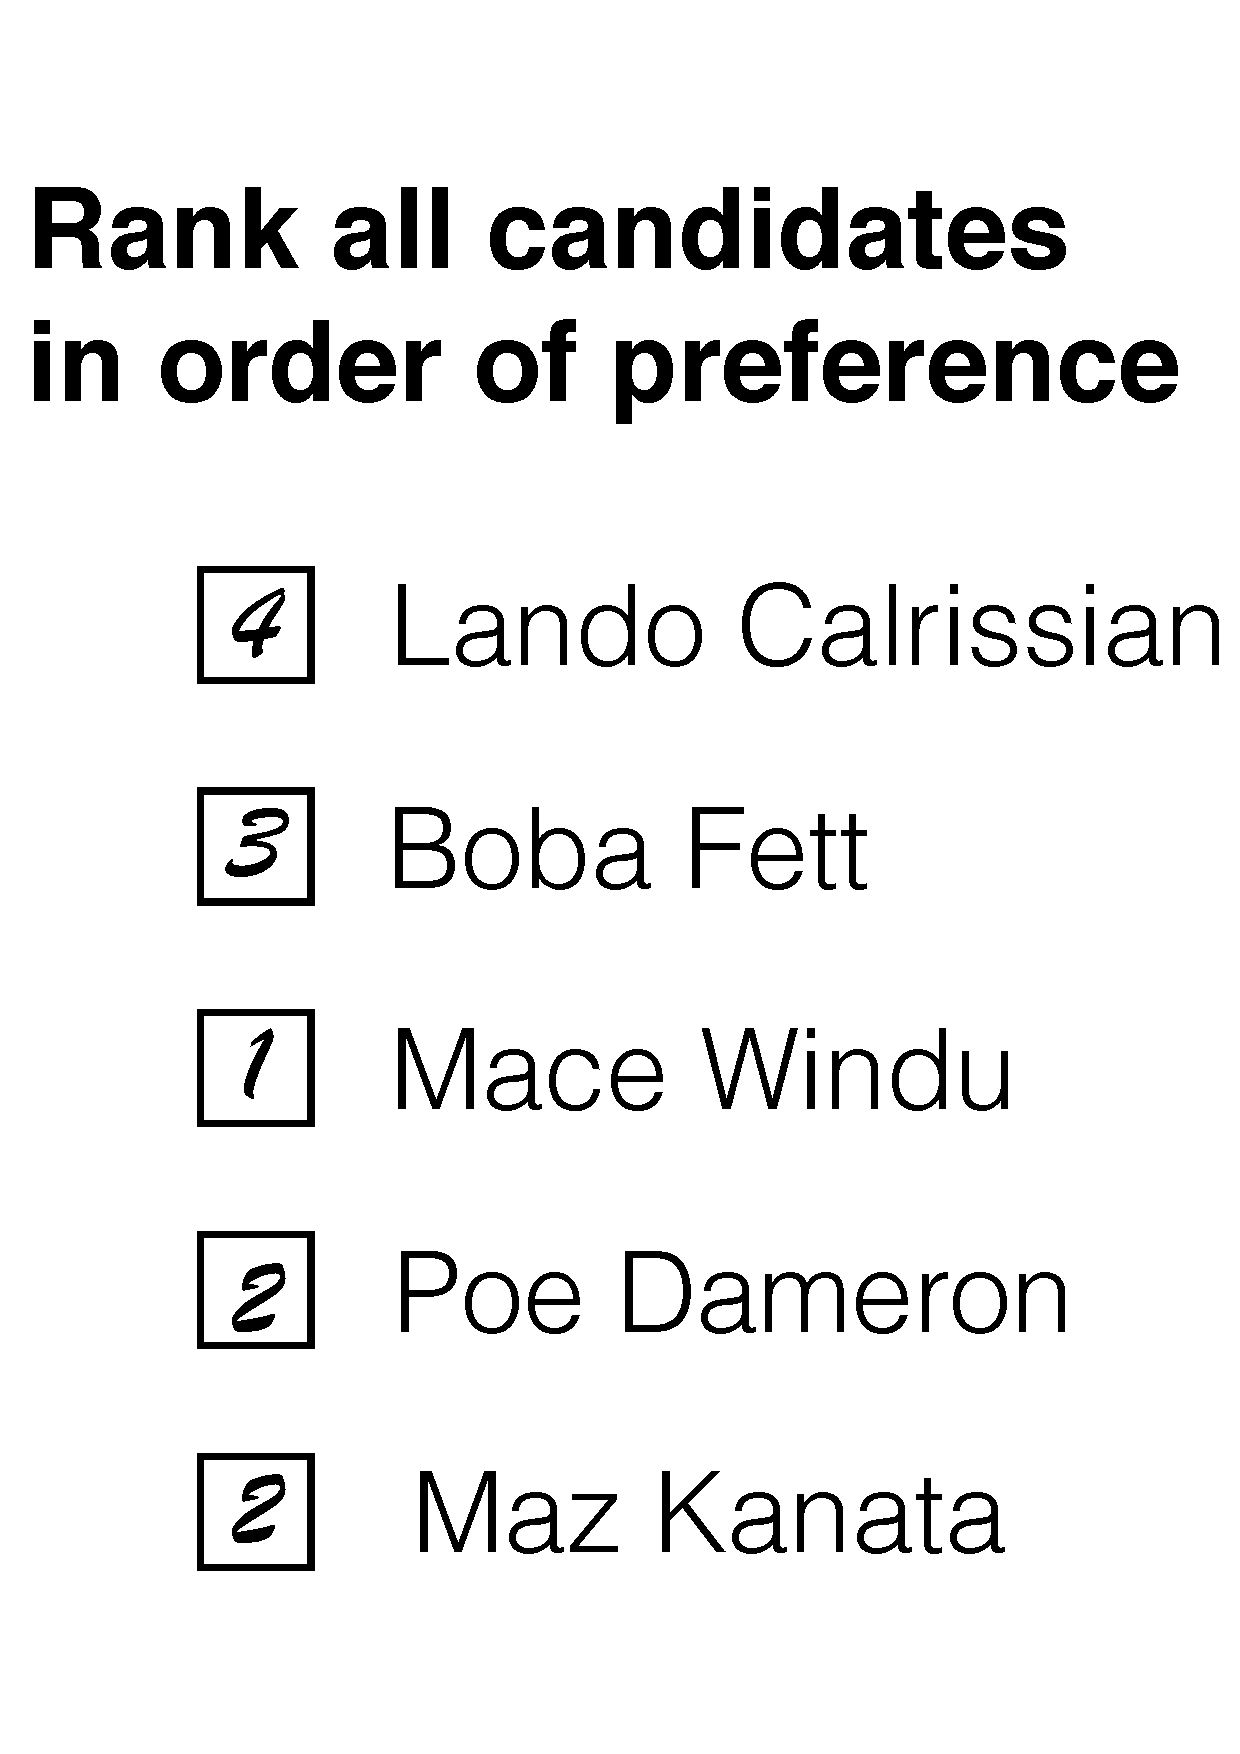
\includegraphics[width=0.18\textwidth]{bal-cropped.pdf}
%\end{center}
%\caption{A hypothetical STV ballot}
%\end{figure}

Each specific STV scheme first determines a \emph{quota}, i.e. the (minimal) number of votes that a candidate needs to attract to be elected (often the Droop quota \cite{Droop:1881:MER}). The quota, mostly but not always, depends on the number of ballots cast, and the number of vacancies to fill. Once the quota has been determined, tallying proceeds as follows:
\begin{enumerate}
  \item count all first preference votes
  \item if a candidate's first preference votes are above the quota, this candidate is elected
  \item if an elected candidate has received votes in excess of the quota, the surplus votes are transferred to the next preference 
  %(possibly resulting in more candidates being elected)
  \item if there are still vacancies to fill and no candidate is  being elected, the candidate with the least number of first preference votes is eliminated, and their votes are transferred to the next preference (possibly resulting in more candidates being elected)
  \item the process continues until either all vacancies are filled, or the number of elected and continuing (not yet eliminated) candidates matches the number of vacancies.
  %candidates together with the candidates not yet eliminated matches the number of vacancies.
\end{enumerate}

This informal description is necessarily imprecise, with details
differing widely between jurisdictions. For example, there are
substantial differences in the details of
precisely which excess ballots are being transferred after
candidates have been elected, or  the order in which surplus ballots are
being transferred.

The goal of this paper is to advance formal methods in elections by demonstrating how STV vote counting can be verified in a modular, transparent, and practical feasible way over a minimal computational trust base:  we show how to synthesise efficient and provably correct verifiers for a large class of STV schemes in a modular and almost fully automated. 


%\texttt{Possibly explain transparent and trust base?}
%Goals.
%\begin{itemize}
%  \item verification of computation of an entire family of STV
%  algorithms
%  \item advance the use of formal methods in elections
%  \item minimize the trust base 
%  \item practical feasibility (development / runtime)
%  \item transparency
%\end{itemize}

We achieve this by first giving a formal definition of STV (called \emph{generic STV}) 
that  encompasses the entire family of STV vote counting
schemes. This definition necessarily under-specifies any particular STV vote counting scheme, but fixes both basic data structures and the mode of computation common to all instances of STV. Trustworthiness is achieved by
not verifying the \emph{software} that computes the result, but instead by verifying \emph{evidence} that substantiates the correctness of the count. Evidence records and corresponds to the individual steps taken in the computation of winners 
%(That is, our approach is an instance of verifiable computation \footnote{DP: reference}). 
%The evidence directly corresponds to the individual steps of the count
(and could so also be verified, or spot-checked manually), giving transparency. We minimize the computational trust base by verifying our executables down to the machine level using a combination of HOL \cite{hol} and CakeML \cite{cake}. 

We observe that every instance of STV performs the same \emph{actions} (e.g. count first preferences, transfer a surplus, eliminate a candidate, etc.) where the precise interpretation of action differs. We formalise these actions as rules that advance the state of the count towards a final result. Evidence for an instance of computation then becomes a sequence of rule applications applied to perform this computation. While generic STV abstracts the commonalities, each \emph{instance} of STV formally specifies the
pre- and postconditions for each rule as well as a boolean function that decides whether a rule has been applied correctly. 

Executable evidence verifiers are constructed almost
automatically:  almost all of the ensuing proof obligations are discharged generically, and we fully  automate the subsequent translation into machine-level verified executable using CakeML.



%Approach.
%\begin{itemize}
%  \item formal definition of the family of STV algorithms
%  \item trustworthyness through external (certificate) validation
%  \item verification of certificates, rather than of implementations
%  \item certificates are rule applications
%  \item trustworthyness through trustworthy certificate verifiers
%  \item minimal computational trust base through  cakeml and hol
%  \item practical feasibility through modularity and proof
%  automation
%  \item full automation of of cakeml translation
%  \item automation of discharge of proof obligations
%\end{itemize}

We evaluate our framework by analysing the degree of automation and modularity achieved, and by giving realistic benchmarks results over real-world election data.

In summary, we present a framework that allows us to formally specify instances of STV and sythesise an executable certificate verifier in a modular way that is itself verified down to the machine level.
\section{Evidences}
\label{sec:DataEv}
  
We are motivated to 
%engineer a trustworthy practical  framework to answer the 
tackle the following problem. How can one verify that any execution of any implementation $\mathcal{P}$ whose source code is secret of an arbitrary  known STV algorithm $\mathcal{A}$ correctly computes the end result according to  $\mathcal{A}$?  



To begin 
%with addressing the problem, 
assume $\mathcal{P}$ is an implementation of an algorithm $\mathcal{A}$. We reasonably demand each execution of $\mathcal{P}$ on a given input $x$ consisting of ballots recorded in the election to output the winners $y$ and evidence $\omega$ as claim  for correctness of the execution.  
 Having evidence available for each execution of $\mathcal{P}$ facilitates checking correctness of the computation carried out \emph{independently} of (the source code of) $\mathcal{P}$. Therefore the original problem boils down to how one can verify the evidence of any \emph{instance of computation} with any algorithm $\mathcal{A}$.


  
The evidence as such must be enough informative to provide transparency of tallying and also allow  voters, or at least a large pool of scrutineers, to verify for themselves that the tally is authentically processed as per instructions of the counting scheme  so that winners truly reflect will of the voters. Therefore the question becomes what information is enough  for establishing transparency and verifiability of tallying  and what data structure for recording the information in the evidence we should choose.
\subsection{Characterisation of Evidence} 
A comprehensive analysis of different STV algorithms reveals existence of a common underlying abstract data type among STV algorithms as follows. 
%Each STV scheme operates on the following data.
\begin{itemize}
\item Some ballots to deal with (assuming) recorded as cast by voters. Each ballot is a pair consisting of a list expressing the preference of a voter and a fractional transfer value,
\item a quota which is the least amount of votes needed to attract in order to be elected, 
\item some candidates competing in the election, 
\item some number of vacancies for which candidates compete,
\item \emph{discrete states of computation} which encapsulate necessary  pieces of information needed to transparently know how the tallying has progressed from the beginning to the end and to be able to independently verify its correctness provided access to the information is granted. 
\end{itemize}
There are two kinds of discrete states of computation. Some of them are final states where tallying has reached a halting state by finding the winners of the election. The other consist of non-final ones where bits and pieces of data are manipulated according to counting mechanism of the STV scheme used, to eventually obtain an end result. Each non-final state comprises seven pieces of data: 
\begin{itemize}
 \item\textbf{uncounted ballots} which await being counted,
 \item\textbf{tally} for holding information about the amount of votes that each candidate has hitherto attracted %up to this state of computation,
 \item\textbf{pile} to know the ballots allocated to each candidate, 
 \item\textbf{backlog of elected} candidates who have exceeded the quota and their surplus votes awaits being transferred,
 \item\textbf{backlog of eliminated} ones whose votes awaits transfer,
 \item\textbf{elected candidates} who are the already elected ones,% whose surplus votes must be transferred,
 \item\textbf{continuing candidates} still continuing in the election. 
 \end{itemize}
The non-final and final states specified above provide us with all information one needs. We therefore find a perfect characterisation for evidence. 
\begin{definition}\label{formalEv}
Suppose an STV algorithm $\mathcal{A}$ is given and $Q$, $s$ and $C$ are respectively the quota, number of vacancies and competing candidates in an electon whose counting algorithm is $\mathcal{A}$ . Also assume  $y$ is the output of an execution of $\mathcal{A}$ on an input $x$. By evidence $\hat{\omega}$ for the execution  we mean the quadruple $(Q,s,C,\Omega)$, where $\Omega$ is the chronological sequence of all states of this instance of computation visited from the initial state where $x$ is input to the final state where $y$ is output.   
\end{definition}
\section{The Generic STV  Machine}
\label{sec:Machine}
\setlength{\abovedisplayskip}{0.5em}
\setlength{\belowdisplayskip}{0.5em}
We have already discussed an abstract data type whose values  formally represent evidence. However we do not yet possess an operational semantics for manipulating data to validate evidence.   On one hand, the semantics must be flexible enough to accommodate variations existing in the counting mechanism of STV algorithms so that we can produce verifiers  specifically operating for validation of evidence output by their associated scheme. On the other hand it must facilitate designing and developing the framework modularly while offering automation of synthesising process of verifiers.


In a secondary examination of the STV family, we also identify a general algorithmic mechanism for performing computation on evidence, which realises the \emph{commonalities} among the family members. This generic method comprises seven general actions%~(Figure~\ref{GenSteps})  
~(Definition~\ref{transitions}) corresponding to actions that tally officers take when counting votes.
\begin{definition}[Generic Counting Actions]\label{transitions}
 The following comprise the generic STV counting actions.
 %The generically appearing counting actions in the STV family are the followings. 
%\begin{figure}  
 \begin{itemize}
\item\textbf{count} for counting the uncounted ballots,
\item\textbf{elect} for electing all or some of the electable candidates, 
\item\textbf{transfer-elected} for distributing surplus votes of elected, %candidates, 
\item\textbf{eliminate} to exclude one or some candidates, 
\item\textbf{transfer-removed} to distribute votes of   the eliminated, %candidates, 
\item\textbf{elected-win} for terminating tallying whenever the vacancies are filled or there is no continuing candidate left, 
\item\textbf{hopeful-win} for terminating tallying whenever  the number of already elected and continuing candidates collectively does not exceed the initial vacancies. 
\end{itemize}
%\caption{Generic STV Counting Steps}
%\label{GenSteps}
%\end{figure}
\end{definition}
Each action is constituted of  preconditions on when and how the action comes into effect, and postconditions dictating what effect applying the action brings about by describing the new state to which computation proceeds. In fact, these conditions are the formal counterparts of the legal clauses in the textual specification of the counting scheme which tell tally officers how to proceed with tallying, and they are common between all flavours of STV. 

For example a constant precondition for applying elimination  asserts that there must be no uncounted ballot left and another one declares that no candidate should be electable at the current state of counting. A postcondition of elimination is that once a candidate is excluded from counting, the list of continuing candidates is updated accordingly so that the excluded candidate no longer received votes. Conjunctions of such declarations comprise what an action is and what an application of that action means.


The underlying abstract data type and the universal algorithmic pattern found in STV characterise components of a finite state machine which we call \emph{generic STV}~(Definition\ref{STVMachine}). The set of machine states consist of the discrete states of computation $\mathcal{S}$ mentioned earlier. The seven generic actions given in Definition~\ref{transitions} form the transition labels $\mathcal{T}$ of the machine. Last, the everywhere present pre- and post-conditions which define (content of)  the actions, make a small-step operational semantics for the machine.  
Note that the states of computation recorded in all possible  evidence now become identical with machine states.


\begin{definition}[The generic STV machine]\label{STVMachine}
Let $\mathcal{S}$  and $\mathcal{T}$
be respectively the set of machine states and transition labels.  Also assume for $t\in\mathcal{T}$, $S_{t}$ $=$ $\bigwedge_{\atop{i\leq j_{t}}} \psi_{i}$ 
 where $\psi_{i}$ is the formal specification (in higher-order logic) of a pre- or post-condition of $t$. Then the \emph{generic STV} is the triple $M = \langle \mathcal{S}, \mathcal{T}, (S_t)_{t \in \mathcal{T}} \rangle$.  
\end{definition}
There are nonetheless variations in STV algorithms  which we  recognise  by separate \emph{instantiations} into the machine.  
\subsection{Instantiations of the Machine with Specific STV schemes}
Differences exist between counting algorithms of STV schemes.  For example in the STV used for electing the upper house representatives of the Victoria state of Australia (Victoria STV)~\cite{vic}, distributing votes of an eliminated candidate occurs step by step in order of the magnitude of the fractional values that those votes carry.  Consequently, a pre-condition for applying the action is to first assure that upon each instance of applying transfer-removed action (a) exactly those votes which have the same fractional value are transferred and (b) the transfer happens according to the magnitude order. In contrast, for example, the STV used in the lower house elections of Tasmania state of Australia (Tasmania STV) does not have such precondition simply because votes of an eliminated candidate are transferred in a single application of transfer-removed. There are also variations in postconditions. For example transfer-elected of the ACT STV~\cite{act} used in the lower house elections of the ACT state of Australia requires distributing only the last parcel of surplus votes received by an elected candidate. But Victoria STV specifies transferring all surplus votes of an elected candidate.  


We formally realise variations of STV algorithms by instantiation~(Definition~\ref{STVInst}) of the generic machine. Recall that the semantics of the machine~(Definition~\ref{STVMachine}) is formed by conjunctions of formally specified universally appearing pre- and postconditions in STV algorithms. An instantiation of the machine with an STV algorithm $\mathcal{A}$ happens by enriching the generic semantics by adding formal specifications of the legal clauses that are specific to $\mathcal{A}$. We hence come to define an operational semantics functioning in accordance with instructions of $\mathcal{A}$. 
\begin{definition}[Instantiation of the Machine]\label{STVInst}
Assume the generic machine $M = \langle \mathcal{S}, \mathcal{T}, (S_t)_{t \in \mathcal{T}} \rangle$ as in Definition~\ref{STVMachine}. An instantiation $\hat{\mathcal{A}}$ for an STV algorithm $\mathcal{A}$ of  the generic STV machine $M$ is a triple $\langle \mathcal{S}, \mathcal{T}, (S'_t)_{t \in \mathcal{T}} \rangle$, where for each $t\in\mathcal{T}$, $S'_{t}$ $=$ $S_{t}\wedge\bigwedge_{\atop{i\leq j'_{t}}} \phi_{i}$. Each $\phi_{i}$ is the formal specification of a pre- or postcondition specific to $\mathcal{A}$.   
\end{definition}

The operational semantics of each instantiation allows  to perform operations such as validation on evidence. Definition~\ref{verifier} lays down what verifying an evidence amounts to. Informally speaking, to check if  evidence is valid one simply needs to inspect if transitions  between each two consecutive states of computation appearing in the evidence occur by a legitimate application of a counting action of the scheme used.

\begin{definition}[verifier]\label{verifier}
Assume $\hat{\mathcal{A}}= \langle \mathcal{S}, \mathcal{T}, (S'_t)_{t \in \mathcal{T}} \rangle$ is an instantiation of the STV algorithm $\mathcal{A}$. A verifier for instances of computation of $\mathcal{A}$ is a function $\hat{\mathcal{V}}$ mapping from $\mathbb{Q}\times\mathbb{N}\times 2^{C}\times$ \textsf{List}$(\mathcal{S})$ to $\{0,1\}$ such that for any evidence $\hat{\omega} = (Q,s,C,\Omega)$ where $\Omega=\langle\Omega_{1},\dots,\Omega_{n}\rangle$, $\hat{\mathcal{V}}(\hat{\omega}) = 1$ if and only if the following holds:\\
$\forall i\in\{1,\dots,n-1\}.$ 
%\hspace*{0.2cm}$\forall \Omega_{i-1}$ $\Omega_{i}\in\mathcal{S}.$
%$\exists \Omega_{1}$ $\Omega_{2}\in$ \textsf{List} $(\mathcal{S}).$ $\Omega = \Omega_{1} + [\Omega_{i-1};\Omega_{i}] + \Omega_{2}$  
$\exists t\in\mathcal{T}.$  $(\Omega_{i-1},\Omega_{i})\in t$ $\wedge~\vdash S'_{t}[\Omega_{i-1},\Omega_{i}]$\\ 
where $\mathbb{Q}$ and $\mathbb{N}$ respectively represent the set of rational and natural numbers, $2^{C}$ is the set of all subsets of $C$, and \textsf{List}$(\mathcal{S})$ is the set of all possible lists of machine states. $\Omega_{i-1}$ is a pre-state and $\Omega_{i}$ is a post-state visited in the execution. The last line means that pre- and post-conditions  of applying $t$ to move from $\Omega_{i-1}$ to $\Omega_{i}$  are logically true. 
\end{definition} 
We shall next provide an example to concretely illustrate a piece of evidence and exemplify how STV schemes work. 
 \subsection{An Example of a Concrete Piece of Evidence}
\label{subsec:InstEv}
Figure~\ref{EvInst} depicts evidence of a small election whose counting algorithm is the ACT STV 
with three candidates $a$, $b$ and $c$, and initially recorded ballots containing
$b_1=([a,c],1/1)$, $b_2=([a,b,c],1/1)$, $b_3=([a,c,b],1/1)$,
$b_4=([b,a],1/1)$, $b_5=([c,b,a],1/1)$.  The first component of each ballot is a preference-ordered list of candidates, and the second is the fractional transfer value (initially set to $1/1$). The evidence consists of a \emph{header} that specifies the quota (computed according to the ACT STV instructions), the number of vacancies, and the list of competing candidates. 
The fourth line is the election result, and the remainder of the evidence are non-final states visited to compute this
outcome. Each non-final state shows uncounted ballots, tallies of candidates, piles of votes attracted, backlog of the elected, backlog of the eliminated, list of elected candidates, and list of continuing candidates. 

First preferences for each candidate are computed. Ballots counted in favour of particular candidates are placed onto that candidate’s pile. In this election, $a$ is the first preference on $b_{1}$, $b_{2}$, and $b_{3}$, $b$ receives $b_{4}$, and $c$ receives $b_{5}$. Tallies are updated so that tally of $a$ becomes 3, and $b$
and $c$ each reach $1/1$. As $a$ exceeds the quota, he is elected and the fractional value of his surplus is updated according to the ACT scheme. Then $a$'s surplus is transferred to continuing candidates $b$ and $c$ and votes are counted according to next preferences shown on $a$'s surplus votes. Candidate $b$ and $c$ each attracts one vote. However  neither of them reaches to the quota. Hence the weakest one $b$ is eliminated. As the number of elected and continuing candidates is equal to 
%does not exceed 
the initial vacancies, the election terminates by declaring $a$ and $c$ winners.
\begin{small} 
\begin{figure}[b]
\begin{tabular}{c@{\hspace{2cm}}c} 
\AxiomC{\tiny 8/3} \noLine

\UnaryInfC{\tiny 2} \noLine \UnaryInfC{\tiny $[a,b,c]$} \noLine

\UnaryInfC{\scriptsize [a,c]} \LeftLabel{\tiny hwin}

\UnaryInfC{\tiny [$b_4$,([a,b,c],1/9)]; a\{3/1\} b\{10/9\} c\{11/9\}; a\{[]\} b\{[]\}
c\{[[$b_{5}$,([c],1/9),([c,b],1/9),([c],1/9)]]\}; []; [a]; [c]}

\LeftLabel{\tiny elim} \UnaryInfC{\tiny []; a\{3/1\} b\{10/9\}
c\{11/9\}, a\{[]\} b\{[[$b_4$],[([a,b,c],1/9)]]\}
c\{[[$b_5$],[([a,c],1/9),([a,c,b],1/9)]]\}; []; [a]; [b,c]}

\LeftLabel{\tiny count} \UnaryInfC{\tiny
[([a,c],1/9),([a,b,c],1/9),([a,c,b],1/9)]; a\{3/1\}
b\{1/1\} c\{1/1\}; a\{[]\} b\{[[$b_4$]]\} c\{[[$b_5$]]\}; []; [a]; [b,c]}

\LeftLabel{\tiny tr-elect} \UnaryInfC{\tiny []; a\{3/1\} b\{1/1\}
 c\{1/1\}; a\{[[([a,c],1/9),([a,b,c],1/9),([a,c,b],1/9)]]\}
b\{[[$b_4$]]\} c\{[[$b_5$]]\}; [a]; [a]; [b,c]} \LeftLabel{\tiny elect}

\UnaryInfC{\tiny []; a\{3/1\} b\{1/1\} c\{1/1\}; a\{[[$b_1$,$b_2$,$b_3$]]\}
b\{[[$b_4$]]\} c\{[[$b_5$]]\}; []; []; [a,b,c]} \LeftLabel{\tiny count}

\UnaryInfC{\tiny ba; a\{0/1\} b\{0/1\} c\{0/1\}; a[] b[] c[]; []; [];
[a,b,c]} \DisplayProof \end{tabular} \caption{An example of  Evidence} \label{EvInst} \end{figure} \end{small}

\section{The Framework Architecture}\label{sec:Arc} 
We progress through three macro-level phases to develop the framework. For the first phase we use HOL4 to formally specify, implement and verify the generic STV, its instantiations, verifiers, and every auxiliary assertions needed for these ends. The second step relies on the verified proof translation tool of CakeML to provably correctly translate implementations of the first phase into equivalent CakeML implementations. The last phase uses the ecosystem of CakeML and its verified compiler to generate machine executable evidence verifiers.   


Figure~\ref{PicArc} is a simplified schematic illustration of the framework modules and their dependencies. We explain the purpose of each and then describe how they collectively function.

\paragraph*{\textbf{Auxiliary}} The module contains specification, implementation and verification of the generic STV. It consists of subdivisions for formal specification of the machine and its components, implementation of functions  meant to be the computational counterparts of the specifications and verification of the implementations by proving that they logically satisfy their respective specifications. Moreover we include specification, implementation and verification of helper assertions which appear in many well-known STV schemes here so that Auxiliary also serves as a comprehensive library for STV. 
\paragraph*{\textbf{Instantiations}}
  Instantiations of the generic STV happen in separate modules which we have schematically shown only two, namely   \textbf{STV}$_{1}$ and \textbf{STV}$_{2}$. An instantiation module \textbf{STV}$_{i}$ for an algorithm $\mathcal{A}$ consists of a subdivision for specification $\hat{\mathcal{A}}_{spec}$ of  the scheme and another one its implementation $\hat{\mathcal{A}}_{dec}$. 
\paragraph*{\textbf{Proofs}} We prove that for an algorithm $\mathcal{A}$ in the above modules,  $\hat{\mathcal{A}}_{dec}$ is logically equivalent to $\hat{\mathcal{A}}_{spec}$. We automate proofs so that they work for various instantiations. 
\paragraph*{\textbf{Verifier}} This module formally realises  the notion of verifier in Definition~\ref{verifier}. However, it is developed in a way that automatically operates  regardless of which STV algorithm is instantiated into the machine. It has three subdivisions. A  specification $\hat{\mathcal{V}}_{spec}$ defining what a verifier is, the implementation $\hat{\mathcal{V}}_{dec}$ and proofs of equivalence of $\hat{\mathcal{V}}_{spec}$ and $\hat{\mathcal{V}}_{dec}$.
\paragraph*{\textbf{Translation}} We translate each implementation $\hat{f}_{imp}$ in HOL4 to a proven  equivalent implementation $f_{\tau}$ in CakeML's environment by using the verified proof translator of CakeML. For example, an implementation  $\hat{\mathcal{A}}_{imp}$ of a scheme $\mathcal{A}$ and its   verifier $\hat{\mathcal{V}}_{imp}$ are  respectively translated into $\mathcal{A}_{\tau}$  and $\mathcal{V}_{\tau}$. 
\paragraph*{\textbf{DeepSpec}} 
For any translated verifier $\mathcal{V}_{\tau}$ and the translated evidence parser $\mathcal{P}_{\tau}$, we obtain logically equivalent deep CakeML embeddings  $\mathcal{V}^{*}$ and $\mathcal{P}^{*}$, respectively. We then use them to establish end-to-end desired properties, based on CakeML's I/O model, about the interaction of the executable verifier with its hosting operating system.   
\tikzset{
    state/.style={
           rectangle,
           rounded corners,
           draw=black, 
           minimum height=2em,
           inner sep=2pt,
           text centered,
           },
}
\begin{figure}[t]
\centering
%\framebox[\columnwidth]{
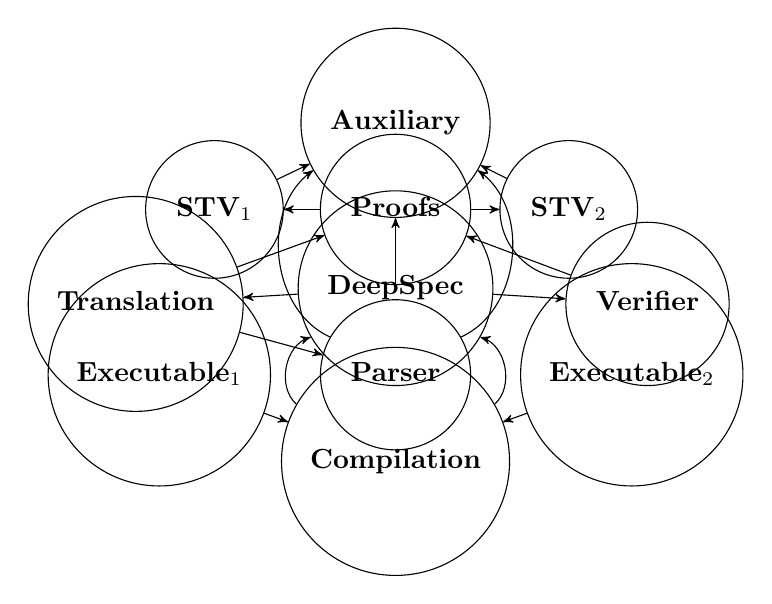
\begin{tikzpicture}[->,>=stealth']

 % Position of PARAM 
 % Use previously defined 'state' as layout (see above)
 % use tabular for content to get columns/rows
 % parbox to limit width of the listing
 \node[state] (Aux) 
 {\begin{tabular}{l}
  \textbf{Auxiliary}
 \end{tabular}};
 
  % STATE STVONE
 \node[state,
  below of=Aux,
  %yshift = -2cm,
  node distance=1.1cm,
  anchor=center] (proof) 
 {%
 \begin{tabular}{l}
  \textbf{Proofs}
 \end{tabular}
 }; 
  
   % STATE PARAM
 \node[state,
  left of= proof,
  xshift = -1.3cm,
  %node distance=1.5cm,
  anchor=center] (STV1) 
 {%
 \begin{tabular}{l}
  \textbf{STV$_{1}$}
 \end{tabular}
 }; 
 
  % STATE STVTWO
 \node[state,
  right of= proof,
  xshift = 1.2cm,
  %node distance=1.5cm,
  anchor=center] (STV2) 
 {%
 \begin{tabular}{l}
  \textbf{STV$_{2}$}
 \end{tabular}
 };
   % STATE EXETWO
 \node[state,
  below of= STV2,
  xshift = 1cm,
  node distance=1.2cm,
  anchor=center] (V) 
 {%
 \begin{tabular}{l}
  \textbf{Verifier}
 \end{tabular}
 };  

   \node[state,
  below of= STV1,
  xshift = - 1cm,
  node distance=1.2cm,
  anchor=center] (T) 
 {%
 \begin{tabular}{l}
  \textbf{Translation}
 \end{tabular}
 };  
 
 \node[state,
  below of = proof,
   %xshift = 3cm,
   node distance = 1cm,
  anchor=center
  %text width=2.5cm
  ] (Deep) 
 {%
 \begin{tabular}{l}
  \textbf{DeepSpec}
%  \parbox{1.7cm}{}
 \end{tabular}
 };
 
  \node[state,
  below of = Deep,
   %xshift = 3cm,
   node distance = 1.1cm,
  anchor=center
  %text width=2.5cm
  ] (parser) 
 {%
 \begin{tabular}{l}
  \textbf{Parser}
%  \parbox{1cm}{}
 \end{tabular}
 };

 \node[state,
  below of = parser,
   %xshift = 3cm,
   node distance = 1.1cm,
  anchor=center] (comp)
  %text width=2.5cm
   {%
 \begin{tabular}{l}
  \textbf{Compilation}
  %\parbox{2cm}{}
 \end{tabular}
 };
 
  \node[state,
  left of = parser,
   xshift = -2cm,
  % node distance = 1.7cm,
  anchor=center
  %text width=2.5cm
  ] (Exe1) 
 {%
 \begin{tabular}{l}
  \textbf{Executable$_{1}$}
  %\parbox{2.5cm}{}
 \end{tabular}
 };
 
 \node[state,
  right of = parser,
   xshift = 2cm,
  % node distance = 1.7cm,
  anchor=center
  %text width=2.5cm
  ] (Exe2) 
 {%
 \begin{tabular}{l}
  \textbf{Executable$_{2}$}
  %\parbox{2cm}{}
 \end{tabular}
 };

 % draw the paths and and print some Text below/above the graph 
 

 \path (proof)     edge (Aux)
       (STV1)     edge (Aux)
       (STV2) edge (Aux)
       (proof) edge (STV1)
       (proof) edge (STV2)
       (V) edge (proof)
       (Deep) edge (V)
       (T) edge (parser)
       (comp) edge [bend left = 60] node[anchor=north,above]{} (Deep)
       (comp) edge [bend right= 60] node[anchor=north,above]{} (Deep)
      (Exe1) edge  (comp) 
      (Exe2) edge (comp)
       (T) edge (proof)
       (Deep) edge (T)
       (parser) edge [bend left = 60] node[anchor=north,above]{} (Aux)
       (parser) edge [bend right= 60] node[anchor=north,above]{} (Aux);
       
\end{tikzpicture}
\caption{Architecture of the Framework, note that direction of arrow represents module dependencies}
\label{PicArc}
\end{figure}
\paragraph*{\textbf{Compilation}} 
Instantiations of CakeML's  compiler for generating machine executable verifiers happen in this module. For any deeply embedded $\mathcal{V}^{*}_{i}$, corresponding to $\hat{\mathcal{V}}_{dec}$ in \textbf{STV}$_{i}$, using proofs  established in \textbf{DeepSpec}, we instantiate the compiler to synthesise executable  verifier $\mathcal{V}_{i}$.  
\section{The Generic STV Formalised}\label{sec:GenCertVer}
We proceed through three steps, namely specification, implementation and verification of implementations in HOL4 to formally verify the machine and its components.
\paragraph*{Specification}  
Recall that we require minimising the trusted computing base  for computing with generated verifiers. The specification module consists of properties which we can use to verify that our implementations of  STV algorithms in HOL4 indeed match with the description of the counting methods used.  
 In light of Definition~\ref{STVMachine} these properties   actually form the semantics of the generic STV machine.   
\paragraph*{Implementation} Our final objective for creating the framework is to produce means for validating concrete evidences. To this end, we need decision procedures used for deciding whether or not a given evidence is valid. Therefore we define boolean-valued functions in the implementation sub-module to computationally realise logical declarations in the specification module. In particular, we implement decision procedures whose computational content  provably realises the specification of the machine semantics.  
\paragraph*{Verification} Here we formally prove that the implementations meet the expectations of their respective specifications. Therefore through verification we come to eliminate a trusted layer  required to lay in our framework.  


We also have another motivation for developing the auxiliary module through this three-part process of specification, implementation and then verification. Familiarity, but no expertise, with our framework and its general purpose is needed for extending it to synthesise an executable verifier for one's desired STV scheme. On the one hand, an average user may lack enough skills in grasping functional programming style which we rely on for implementing verifiers in HOL4. However, the same user most probably has had exposure to formulations of mathematical properties  in first-order logic syntax. Including purely descriptive logical assertions as our specifications, proven equivalent to their implementations, facilitates the users with means to understand the functionality of components, modules and the system as a whole simply by inspecting the specifications instead of implementations.
\subsection{Data Structure of Machine States}
\label{MachineData}
 We choose the data structure  given in Definition~\ref{judgement} for implementing the abstract data type underlying the generic STV.  We have four reasons for this choice of data structure. 
 \begin{itemize}
\item As the abstract syntactic representation of evidence closely represents concrete evidences, designing the parser and inspecting  its  correctness is less challenging.  
 \item HOL4 has well developed libraries comprised of verified assertions of operations on list structure. By structuring the data on lists, we facilitate us and users  with exploitation of  already verified tools to formalise the framework and avoid inventing the unnecessary from the scratch. 
 \item HOL4 also has well-developed tactics for discharging proof obligations on assertions involving list structure and operations on it. We therefore come to provide us with means for ease of verification of the formalised assertions.
 \item Understanding the data structure used in the  framework implementation is critical for ease of  its usability and extensibility by third parties.  The type $\mathit{judgement}$ closely models concrete evidences such as the one in figure~\ref{EvInst}. Therefore one can sensibly perceive the  abstraction step taken for modelling  concrete data which in turn enhances understandability of the framework and its mechanism. 
   \end{itemize}
\begin{definition}\label{judgement}
We formalise machine states as an inductive type  $\mathit{judgement}$ whose constructors are  $\mathit{NonFinal}$ and $\mathit{Final}$. 
 A $\mathit{Final~(w)}$ judgement declares $w$ as winners of the election. A  $\mathit{NonFinal~(ba,t,p,bl_{1},bl_{2},e,h)}$ judgement  consists of uncounted ballots $ba$, tally $t$, pile $p$, $bl_{1}$ the backlog of elected candidates, $bl_{2}$ the backlog of eliminated candidates, and $e$ and $h$ for the list of elected and continuing~(hopeful) candidates. 
\begin{holthmenv}
\HOLTyOp{judgement}\;=\\
\;\;\;\;\HOLConst{NonFinal}\;(\HOLTyOp{ballots}\;\HOLTokenProd{}\;\HOLTyOp{tallies}\;\HOLTokenProd{}\;\HOLTyOp{piles}\;\HOLTokenProd{}\\\;\;\;\;\;\;\HOLTyOp{cand}\;\HOLTyOp{list}\;\HOLTokenProd{}\;\HOLTyOp{cand}\;\HOLTyOp{list}\;\HOLTokenProd{}\;\HOLTyOp{cand}\;\HOLTyOp{list}\;\HOLTokenProd{}\;\HOLTyOp{cand}\;\HOLTyOp{list})\\
\;\;\HOLTokenBar{}\;\HOLConst{Final}\;(\HOLTyOp{cand}\;\HOLTyOp{list})
\end{holthmenv} 
 The types  $\mathit{ballots}$, $\mathit{tallies}$ and $\mathit{piles}$ are respectively abbreviations for  $\mathit{((cand ~list)\times rat) list}$,   $\mathit{(cand\times rat)~list}$ and $\mathit{(cand\times(ballots~list)~list) ~list}$ where $\mathit{rat}$ is the HOL4 type of fractional numbers.
\end{definition}
 Recall that objects whose type is $\mathit{piles}$ serve as containers for recording the ballots allocated to each candidate. Our choice for type of piles allows us to store the ballots received by each candidate in chunks of lists rather than one single list containing all of them.  We have two reasons for designing the type of piles as it stands instead of $\mathit{(cand\times(ballots~list))~list}$;  
\paragraph*{(a)} Some STV schemes such as the lower house ACT and Tasmania STV, employ a notion called ''last parcel''. In short the last parcel of a candidate is the collection of those ballots received by the candidate at the last round of application of the count transition which made the tally of the candidate reach or exceed the quota and therefore be elected.  Only the last parcel, instead of all, of an elected candidate is distributed, according to next preferences shown on the ballots in the last parcel, to the continuing candidates.
%the ballots received by the candidate.
 Also  they update the fractional transfer value, that each ballot in the last parcel  awaiting transfer carries, based on the length of the last parcel. To  accommodate this notion and its effect, we need identifying the ballots constituting the last parcel of an elected. We hence formalise the pile to record, for each  continuing candidate, a list consisting of lists of ballots each received upon  chronological applications of count transition.  Once a candidate is elected their pile may be manipulated differently from the continuing candidates. 
\paragraph*{(b)} We noted earlier that the STV used for the upper house elections in the Victoria state transfers votes of an eliminated candidate chunk by chunk in several applications of transfer-removed, rather than in a single action, in order of the magnitude of the fractional value that the chunks carry. We therefore need to rearrange the pile of ballots of an eliminated candidate into lists based on equality of the fractional value of ballots and then distribute them in the proper order as the scheme requires. This means that the type of piles has to be as it is defined above.   
Implementing piles in this way enables us to tailor the semantics of the transfer and elect transitions and their instantiations in such a way to modularly formalise several STV schemes which use the last parcel or stepwise distribution of votes form eliminated candidates or the combination of both. 


There is also a reason for choosing the type $rat$  
%as the underlying arithmetic for the formalisation, 
instead of e.g. floating numbers. Elections with an STV counting scheme have a small margin of victory especially for the last vacancy left to fill \cite{MBlo}. This margin may happen to be less than magnitude of the error caused by accumulation of rounding errors as it is with floating points.  Hence one must sensibly avoid the high  cost of electing a wrong candidate by falling into traps of imprecise calculations due to unintelligent choices. Using exact fractions allows safe handling of calculations. 
\subsection{The Semantics and its Auxiliary Components}
\label{sec:MachineSem}

The semantics of each machine transition label consists of conjunctions of formally specified general pre- and post-conditions across STV schemes which enforce when and how to take a tallying action and what the immediate effect is. To demonstrate the process of specification, implementation and verification of the machine transitions and their semantics, we discuss the transfer-elected transition.


STV schemes \emph{explicitly} declare four conditions that must be satisfied  for any legitimate application of transfer-elected; 
\begin{itemize}
\item[a.] there are still vacancies to fill
\item[b.] There are no uncounted ballots to deal with
%\item[c.] no more continuing candidate other than already elected has reached or exceeded the quota
\item[c.] there is no vote from any eliminated candidate still awaiting distribution, and
\item[d.] there are surplus votes of elected candidates to  transfer.
\end{itemize}


Also there are some \emph{implicit} conditions present in legal documents describing transfer-elected. These constraints come to attention either as the result of a straightforward understanding of the explicit conditions above or as   auxiliary components that are taken for granted by legislators but are
necessary for proper functioning of the explicit constraints;
\begin{enumerate}
\item every candidate in the pre- and post-state of transfer-elected has a unique tally and pile
\item no one is elected or eliminated by applying transfer-elected
\item no candidate attracts any new vote by transfer-elect and therefore tallies remain the same
\item candidates whose names appears in the backlog of elected are indeed among elected candidates
\item any elected candidate is no longer a continuing candidate so that they do not receive votes any further
\item the list of competing candidates in the election is not empty and has no duplication of names
\end{enumerate}  
Conjunctions of formal declarations of the above explicit and implicit conditions form the semantics of the transition label transfer-elected.   The predicate TransferAuxSpec defines  the semantics of this transition.
 \begin{small}
\begin{holthmenv}
  \HOLConst{TransferAuxSpec}\;(\HOLFreeVar{qu}\HOLSymConst{,}\HOLFreeVar{st}\HOLSymConst{,}\HOLFreeVar{l})\;\HOLFreeVar{ba}\;\HOLFreeVar{t}\;\HOLFreeVar{t\sp{\prime}}\;\HOLFreeVar{p}\;\HOLFreeVar{p\sp{\prime}}\;\HOLFreeVar{bl}\;\HOLFreeVar{bl\sb{\mathrm{2}}}\;\HOLFreeVar{bl\sb{\mathrm{2}}\sp{\prime}}\;\HOLFreeVar{e}\;\HOLFreeVar{e\sp{\prime}}\;\HOLFreeVar{h}\;\HOLFreeVar{h\sp{\prime}}\;\HOLSymConst{\HOLTokenEquiv{}}\\
\;\;\HOLFreeVar{bl\sb{\mathrm{2}}}\;\HOLSymConst{=}\;\HOLConst{\ensuremath{[\,]}}\;\HOLSymConst{\HOLTokenConj{}}\;\HOLFreeVar{bl}\;\HOLSymConst{\HOLTokenNotEqual{}}\;\HOLConst{\ensuremath{[\,]}}\;\HOLSymConst{\HOLTokenConj{}}\;\HOLFreeVar{ba}\;\HOLSymConst{=}\;\HOLConst{\ensuremath{[\,]}}\;\HOLSymConst{\HOLTokenConj{}}\;\HOLFreeVar{bl\sb{\mathrm{2}}\sp{\prime}}\;\HOLSymConst{=}\;\HOLConst{\ensuremath{[\,]}}\;\HOLSymConst{\HOLTokenConj{}}\;\HOLFreeVar{t\sp{\prime}}\;\HOLSymConst{=}\;\HOLFreeVar{t}\;\HOLSymConst{\HOLTokenConj{}}\;\HOLFreeVar{e\sp{\prime}}\;\HOLSymConst{=}\;\HOLFreeVar{e}\;\HOLSymConst{\HOLTokenConj{}}\\
\;\;\HOLFreeVar{h\sp{\prime}}\;\HOLSymConst{=}\;\HOLFreeVar{h}\;\HOLSymConst{\HOLTokenConj{}}\;\HOLConst{length}\;\HOLFreeVar{e}\;\HOLSymConst{\HOLTokenLt{}}\;\HOLFreeVar{st}\;\HOLSymConst{\HOLTokenConj{}}\;(\HOLSymConst{\HOLTokenForall{}}\HOLBoundVar{d}.\;\HOLConst{\HOLConst{mem}}\;\HOLBoundVar{d}\;(\HOLFreeVar{h}\;\HOLSymConst{\HOLTokenDoublePlus}\;\HOLFreeVar{e})\;\HOLSymConst{\HOLTokenImp{}}\;\HOLConst{\HOLConst{mem}}\;\HOLBoundVar{d}\;\HOLFreeVar{l})\;\HOLSymConst{\HOLTokenConj{}}\\
\;\;(\HOLSymConst{\HOLTokenForall{}}\HOLBoundVar{d}.\;\HOLConst{\HOLConst{mem}}\;\HOLBoundVar{d}\;\HOLFreeVar{bl}\;\HOLSymConst{\HOLTokenImp{}}\;\HOLConst{\HOLConst{mem}}\;\HOLBoundVar{d}\;\HOLFreeVar{l})\;\HOLSymConst{\HOLTokenConj{}}\;\HOLConst{distinct}\;(\HOLFreeVar{h}\;\HOLSymConst{\HOLTokenDoublePlus}\;\HOLFreeVar{e})\;\HOLSymConst{\HOLTokenConj{}}\\
\;\;\HOLConst{Valid_PileTally}\;\HOLFreeVar{t}\;\HOLFreeVar{l}\;\HOLSymConst{\HOLTokenConj{}}\;\HOLConst{Valid_PileTally}\;\HOLFreeVar{p}\;\HOLFreeVar{l}\;\HOLSymConst{\HOLTokenConj{}}\;\HOLConst{Valid_PileTally}\;\HOLFreeVar{p\sp{\prime}}\;\HOLFreeVar{l}\;\HOLSymConst{\HOLTokenConj{}}\\\;\;\HOLConst{ValidInitCandList}\;\HOLFreeVar{l}\;\HOLSymConst{\HOLTokenConj{}}
\;\;\HOLConst{distinct}\;(\HOLConst{map}\;\HOLConst{fst}\;\HOLFreeVar{t})\;\HOLSymConst{\HOLTokenConj{}}\;\HOLConst{distinct}\;(\HOLConst{map}\;\HOLConst{fst}\;\HOLFreeVar{p})
\end{holthmenv}
\end{small}

Transfer-elect, as is the case for other formalised transitions, is parametrised by the quota $qu$, number of initial vacancies $st$ and the list $l$ of all candidates competing in the election. The semantics of the transition declares that given the ballots $ba$, tally $t$, pile $p$, backlog of elected $bl$, backlog of eliminated $bl_{2}$ and the list of elected $e$ and continuing candidates $h$ in the pre-state of transfer-elected, and their respective counterparts in the post-state characterised by having a prime symbol, some conditions as specified above are satisfied by the transition.  Note that \textsf{mem} in Definition of TransferAuxSpec declares list membership. 
  
   
  
\begin{small}
\begin{holthmenv}
  \HOLConst{ValidInitCandList}\;\HOLFreeVar{l}\;\HOLSymConst{\HOLTokenEquiv{}}\;\HOLFreeVar{l}\;\HOLSymConst{\HOLTokenNotEqual{}}\;\HOLConst{\ensuremath{[\,]}}\;\HOLSymConst{\HOLTokenConj{}}\;\HOLConst{distinct}\;\HOLFreeVar{l}
\end{holthmenv}
\end{small}
The predicate ValidInitCandList which realises item (6) asserts that each candidate has a pile and a tally. We also declare that elements in the first component of the tally $t$ and pile $p$ are distinct. Therefore we come to satisfy item (1).
\begin{small}
\begin{holthmenv}
  \HOLConst{Valid_PileTally}\;\HOLFreeVar{t}\;\HOLFreeVar{l}\;\HOLSymConst{\HOLTokenEquiv{}}\;\HOLSymConst{\HOLTokenForall{}}\HOLBoundVar{c}.\;\HOLConst{\HOLConst{mem}}\;\HOLBoundVar{c}\;\HOLFreeVar{l}\;\HOLSymConst{\HOLTokenEquiv{}}\;\HOLConst{\HOLConst{mem}}\;\HOLBoundVar{c}\;(\HOLConst{map}\;\HOLConst{fst}\;\HOLFreeVar{t})
\end{holthmenv}
\end{small}
We implement for each of the above declarations a counterpart 
%computational 
\underline{dec}ision procedure that is later translated and then extracted as part of the verifier for actual computation. To illustrate how this phase proceeds, we provide some instances. The following two functions together implement Valid\textunderscore{}PileTally.
\begin{small}
\begin{holthmenv}
  \HOLConst{Valid_PileTally_dec1}\;\HOLConst{\ensuremath{[\,]}}\;\HOLFreeVar{l}\;\HOLSymConst{\HOLTokenEquiv{}}\;\HOLConst{true}\\
\HOLConst{Valid_PileTally_dec1}\;(\HOLFreeVar{h}\HOLSymConst{::}\HOLFreeVar{t})\;\HOLFreeVar{l}\;\HOLSymConst{\HOLTokenEquiv{}}\\
\;\;\HOLConst{\HOLConst{mem}}\;(\HOLConst{fst}\;\HOLFreeVar{h})\;\HOLFreeVar{l}\;\HOLSymConst{\HOLTokenConj{}}\;\HOLConst{Valid_PileTally_dec1}\;\HOLFreeVar{t}\;\HOLFreeVar{l}
\end{holthmenv}
\end{small}
\begin{small}
\begin{holthmenv}
  \HOLConst{Valid_PileTally_dec2}\;\HOLFreeVar{t}\;\HOLConst{\ensuremath{[\,]}}\;\HOLSymConst{\HOLTokenEquiv{}}\;\HOLConst{true}\\
\HOLConst{Valid_PileTally_dec2}\;\HOLFreeVar{t}\;(\HOLFreeVar{l\sb{\mathrm{0}}}\HOLSymConst{::}\HOLFreeVar{ls})\;\HOLSymConst{\HOLTokenEquiv{}}\\
\;\;\HOLKeyword{if}\;\HOLConst{\HOLConst{mem}}\;\HOLFreeVar{l\sb{\mathrm{0}}}\;(\HOLConst{map}\;\HOLConst{fst}\;\HOLFreeVar{t})\;\HOLKeyword{then}\;\HOLConst{Valid_PileTally_dec2}\;\HOLFreeVar{t}\;\HOLFreeVar{ls}\;
\HOLKeyword{else}\;\HOLConst{false}
\end{holthmenv}
\end{small}
We prove that the implementations and specification match:
\begin{small}
\begin{holthmenv}
  \HOLConst{Valid_PileTally}\;\HOLFreeVar{t}\;\HOLFreeVar{l}\;\HOLSymConst{\HOLTokenEquiv{}}\\
\;\;\HOLConst{Valid_PileTally_dec1}\;\HOLFreeVar{t}\;\HOLFreeVar{l}\;\HOLSymConst{\HOLTokenConj{}}\;\HOLConst{Valid_PileTally_dec2}\;\HOLFreeVar{t}\;\HOLFreeVar{l}
\end{holthmenv}
\end{small}
Conjunctions of the computational implementations  define a computational twin TransferAuxDec for the specification  of the transfer-elected semantics TransferAuxSpec. 
\begin{small}
\begin{holthmenv}
  \HOLConst{TransferAuxDec}\;(\HOLFreeVar{qu}\HOLSymConst{,}\HOLFreeVar{st}\HOLSymConst{,}\HOLFreeVar{l})\;\HOLFreeVar{ba}\;\HOLFreeVar{t}\;\HOLFreeVar{t\sp{\prime}}\;\HOLFreeVar{p}\;\HOLFreeVar{p\sp{\prime}}\;\HOLFreeVar{bl}\;\HOLFreeVar{bl\sb{\mathrm{2}}}\;\HOLFreeVar{bl\sb{\mathrm{2}}\sp{\prime}}\;\HOLFreeVar{e}\;\HOLFreeVar{e\sp{\prime}}\;\HOLFreeVar{h}\;\HOLFreeVar{h\sp{\prime}}\;\HOLSymConst{\HOLTokenEquiv{}}\\
\;\;\HOLConst{null}\;\HOLFreeVar{bl\sb{\mathrm{2}}}\;\HOLSymConst{\HOLTokenConj{}}\;\HOLFreeVar{e\sp{\prime}}\;\HOLSymConst{=}\;\HOLFreeVar{e}\;\HOLSymConst{\HOLTokenConj{}}\;\HOLFreeVar{h\sp{\prime}}\;\HOLSymConst{=}\;\HOLFreeVar{h}\;\HOLSymConst{\HOLTokenConj{}}\;\HOLFreeVar{t\sp{\prime}}\;\HOLSymConst{=}\;\HOLFreeVar{t}\;\HOLSymConst{\HOLTokenConj{}}\;\HOLConst{length}\;\HOLFreeVar{e}\;\HOLSymConst{\HOLTokenLt{}}\;\HOLFreeVar{st}\;\HOLSymConst{\HOLTokenConj{}}\\
\;\;\HOLConst{list_MEM_dec}\;(\HOLFreeVar{h}\;\HOLSymConst{\HOLTokenDoublePlus}\;\HOLFreeVar{e})\;\HOLFreeVar{l}\;\HOLSymConst{\HOLTokenConj{}}\;\HOLConst{list_MEM_dec}\;\HOLFreeVar{bl}\;\HOLFreeVar{l}\;\HOLSymConst{\HOLTokenConj{}}\\
\;\;\HOLConst{distinct}\;(\HOLFreeVar{h}\;\HOLSymConst{\HOLTokenDoublePlus}\;\HOLFreeVar{e})\;\HOLSymConst{\HOLTokenConj{}}\;\HOLConst{Valid_PileTally_dec1}\;\HOLFreeVar{t}\;\HOLFreeVar{l}\;\HOLSymConst{\HOLTokenConj{}}\\
\;\;\HOLConst{Valid_PileTally_dec2}\;\HOLFreeVar{t}\;\HOLFreeVar{l}\;\HOLSymConst{\HOLTokenConj{}}\;\HOLConst{Valid_PileTally_dec1}\;\HOLFreeVar{p}\;\HOLFreeVar{l}\;\HOLSymConst{\HOLTokenConj{}}\\
\;\;\HOLConst{Valid_PileTally_dec2}\;\HOLFreeVar{p}\;\HOLFreeVar{l}\;\HOLSymConst{\HOLTokenConj{}}
\;\HOLConst{Valid_PileTally_dec1}\;\HOLFreeVar{p\sp{\prime}}\;\HOLFreeVar{l}\;\HOLSymConst{\HOLTokenConj{}}\\
\;\;\HOLConst{Valid_PileTally_dec2}\;\HOLFreeVar{p\sp{\prime}}\;\HOLFreeVar{l}\;\HOLSymConst{\HOLTokenConj{}}\;\HOLSymConst{\HOLTokenNeg{}}\HOLConst{null}\;\HOLFreeVar{l}\;\HOLSymConst{\HOLTokenConj{}}\;\HOLConst{distinct}\;\HOLFreeVar{l}\;\HOLSymConst{\HOLTokenConj{}}\;\HOLSymConst{\HOLTokenConj{}}\;\HOLConst{null}\;\HOLFreeVar{bl\sb{\mathrm{2}}\sp{\prime}}\\
\;\;\HOLConst{distinct}\;(\HOLConst{map}\;\HOLConst{fst}\;\HOLFreeVar{t})\;\HOLSymConst{\HOLTokenConj{}}\;\HOLConst{distinct}\;(\HOLConst{map}\;\HOLConst{fst}\;\HOLFreeVar{p})\;\HOLSymConst{\HOLTokenConj{}}\;\HOLSymConst{\HOLTokenNeg{}}\HOLConst{null}\;\HOLFreeVar{bl}\;\HOLSymConst{\HOLTokenConj{}}
\;\HOLConst{null}\;\HOLFreeVar{ba}
\end{holthmenv}
\end{small}

Similarly  
we obtain specification and computational implementation for other machine transitions as well. Then the specification (implementation) of the machine semantics is comprised of the collection of specification (resp. implementation) of the individual transitions. We formally prove 
%formally prove that for 
each transition implementation  matches with its specification.
\begin{theorem}
Assume $M^{spec} = \langle \mathcal{S}, \mathcal{T}, (S_{t}^{spec})_{t \in \mathcal{T}} \rangle$ is the specification of the machine and  $M^{dec} = \langle \mathcal{S}, \mathcal{T}, (S_{t}^{dec})_{t \in \mathcal{T}} \rangle$ is its computational implementation. Then for any $t\in\mathcal{T}$,  $\mathcal{S}_{t}^{spec}\Leftrightarrow\mathcal{S}_{t}^{dec}$.      
\end{theorem}

One can already proceed to synthesise an executable verifier from the machine. Such a verifier can correctly decide if given evidence $\omega$ claimed to have been produced by an algorithm whose counting scheme is STV, instead of e.g. First-Past-The-Post voting~\cite{DFar} where voters choose whom they prefer most and the candidate with the most amount of votes received is elected.  
However we wish to generate verifiers that can recognise and validate according to which specific STV algorithm the evidence $\omega$ has been output. Hence we need to enrich the computational content of the machine semantics with more  pre- and postconditions which are particular to individual STV schemes. We refer to this enrichment process as instantiation of the machine and discuss it further below.
\section{Instantiations of the Machine}\label{sec:InstMachine}
We exemplify how an instantiation of the transfer-elected succeeds for transferring surplus of elected candidates based on the ACT STV.
%\footnote{The Tasmania STV also uses similar surplus transfer mechanism.}.
 Instantiation of other machine transitions proceed in a  similar manner. Under section 'Step 3' and 'transfer surplus from elected candidates' the protocol explains under what conditions and how to distribute surplus votes. We summarise and rephrase these sections as follows. 
\begin{itemize}
\item[$\bullet_{1}$] no  candidate exceeds the quota
%\item[$\bullet_{2}$] ballots received by a candidate are piled in separate chunks called parcels. 
\item[$\bullet_{2}$] the  parcel of an elected with surplus is not empty.
\item[$\bullet_{3}$] distribution of the surplus of an elected candidate proceeds in one single step.
\item[$\bullet_{4}$] surplus of elected candidates is distributed one at a time beginning with those who are elected earlier. 
\item[$\bullet_{5}$] pile of the candidate whose surplus is transferred is emptied in the post-state of transfer-elected.
\item[$\bullet_{6}$] only the last parcel of votes  received (which resulted in a surplus) is transferred. It may be that the last parcel is the only parcel in a candidate's pile (if only one application of the count action has occurred), or more parcels exist (if several actions of count has happened as a result of earlier  elect, transfer or eliminate actions)
\item[$\bullet_{7}$] pile of any candidate other than the one whose surplus is transferred at this stage remains the same.
\item[$\bullet_{8}$] the fractional transfer value is subsequently computed depending on whether or not the last parcel is the only parcel of ballots in the pile of the elected candidate. 
\end{itemize}
\begin{small}
\begin{holthmenv}
  \HOLConst{TransferActSpec}\;(\HOLFreeVar{qu}\HOLSymConst{,}\HOLFreeVar{st}\HOLSymConst{,}\HOLFreeVar{l})\;\HOLFreeVar{j\sb{\mathrm{1}}}\;\HOLFreeVar{j\sb{\mathrm{2}}}\;\HOLSymConst{\HOLTokenEquiv{}}\\
\;\;\HOLSymConst{\HOLTokenExists{}}\HOLBoundVar{ba}\;\HOLBoundVar{ba\sp{\prime}}\;\HOLBoundVar{t}\;\HOLBoundVar{t\sp{\prime}}\;\HOLBoundVar{p}\;\HOLBoundVar{p\sp{\prime}}\;\HOLBoundVar{bl}\;\HOLBoundVar{bl\sp{\prime}}\;\HOLBoundVar{bl\sb{\mathrm{2}}}\;\HOLBoundVar{bl\sb{\mathrm{2}}\sp{\prime}}\;\HOLBoundVar{e}\;\HOLBoundVar{e\sp{\prime}}\;\HOLBoundVar{h}\;\HOLBoundVar{h\sp{\prime}}.\\
\;\;\;\;\HOLFreeVar{j\sb{\mathrm{1}}}\;\HOLSymConst{=}\;\HOLConst{NonFinal}\;(\HOLBoundVar{ba}\HOLSymConst{,}\HOLBoundVar{t}\HOLSymConst{,}\HOLBoundVar{p}\HOLSymConst{,}\HOLBoundVar{bl}\HOLSymConst{,}\HOLBoundVar{bl\sb{\mathrm{2}}}\HOLSymConst{,}\HOLBoundVar{e}\HOLSymConst{,}\HOLBoundVar{h})\;\HOLSymConst{\HOLTokenConj{}}\\
\;\;\;\;\HOLConst{TransferAuxSpec}\;(\HOLFreeVar{qu}\HOLSymConst{,}\HOLFreeVar{st}\HOLSymConst{,}\HOLFreeVar{l})\;\HOLBoundVar{ba}\;\HOLBoundVar{t}\;\HOLBoundVar{t\sp{\prime}}\;\HOLBoundVar{p}\;\HOLBoundVar{p\sp{\prime}}\;\HOLBoundVar{bl}\;\HOLBoundVar{bl\sb{\mathrm{2}}}\;\HOLBoundVar{bl\sb{\mathrm{2}}\sp{\prime}}\;\HOLBoundVar{e}\;\HOLBoundVar{e\sp{\prime}}\;\HOLBoundVar{h}\HOLBoundVar{h\sp{\prime}}\;\HOLSymConst{\HOLTokenConj{}}\\\;\;\;\;(\HOLSymConst{\HOLTokenForall{}}\HOLBoundVar{c\sp{\prime}}.\;\HOLConst{\HOLConst{mem}}\;\HOLBoundVar{c\sp{\prime}}\;\HOLBoundVar{h}\;\HOLSymConst{\HOLTokenImp{}}\;\HOLSymConst{\HOLTokenExists{}}\HOLBoundVar{x}.\;\HOLConst{\HOLConst{mem}}\;(\HOLBoundVar{c\sp{\prime}}\HOLSymConst{,}\HOLBoundVar{x})\;\HOLBoundVar{t}\;\HOLSymConst{\HOLTokenConj{}}\;\HOLBoundVar{x}\;\HOLSymConst{\HOLTokenLt{}}\;\HOLFreeVar{qu})\;\HOLSymConst{\HOLTokenConj{}}\\
\;\;\;\;\;\;\HOLSymConst{\HOLTokenExists{}}\HOLBoundVar{l\sb{\mathrm{1}}}\;\HOLBoundVar{c}.
\;(\HOLBoundVar{bl}\;\HOLSymConst{=}\;\HOLBoundVar{c}\HOLSymConst{::}\HOLBoundVar{l\sb{\mathrm{1}}}\;\HOLSymConst{\HOLTokenConj{}}\;\HOLConst{\HOLConst{mem}}\;\HOLBoundVar{c}\;\HOLFreeVar{l}\;\HOLSymConst{\HOLTokenConj{}}\;(\HOLSymConst{\HOLTokenForall{}}\HOLBoundVar{l\sb{\mathrm{2}}}.\;\HOLConst{\HOLConst{mem}}\;(\HOLBoundVar{c}\HOLSymConst{,}\HOLBoundVar{l\sb{\mathrm{2}}})\;\HOLBoundVar{p}\;\HOLSymConst{\HOLTokenImp{}}\;\HOLBoundVar{l\sb{\mathrm{2}}}\;\HOLSymConst{\HOLTokenNotEqual{}}\;\HOLConst{\ensuremath{[\,]}})\\\;\;\;\;\;\;\HOLSymConst{\HOLTokenConj{}}\;\HOLBoundVar{bl\sp{\prime}}\;\HOLSymConst{=}\;\HOLBoundVar{l\sb{\mathrm{1}}}\;\HOLSymConst{\HOLTokenConj{}}\;\HOLBoundVar{ba\sp{\prime}}\;\HOLSymConst{=}\;\HOLConst{last}\;(\HOLConst{getCandPile}\;\HOLBoundVar{c}\;\HOLBoundVar{p})\;\HOLSymConst{\HOLTokenConj{}}\;\HOLConst{\HOLConst{mem}}\;(\HOLBoundVar{c}\HOLSymConst{,}\HOLConst{\ensuremath{[\,]}})\;\HOLBoundVar{p\sp{\prime}}\;\HOLSymConst{\HOLTokenConj{}}\\
\;\;\;\;\;\;\HOLSymConst{*}\;\HOLSymConst{\HOLTokenForall{}}\HOLBoundVar{d}.
\;\HOLBoundVar{d}\;\HOLSymConst{\HOLTokenNotEqual{}}\;\HOLBoundVar{c}\;\HOLSymConst{\HOLTokenImp{}}\;\HOLSymConst{\HOLTokenForall{}}\HOLBoundVar{l\sb{\mathrm{3}}}.\;(\HOLConst{\HOLConst{mem}}\;(\HOLBoundVar{d}\HOLSymConst{,}\HOLBoundVar{l\sb{\mathrm{3}}})\;\HOLBoundVar{p}\;\HOLSymConst{\HOLTokenImp{}}\;\HOLConst{\HOLConst{mem}}\;(\HOLBoundVar{d}\HOLSymConst{,}\HOLBoundVar{l\sb{\mathrm{3}}})\;\HOLBoundVar{p\sp{\prime}})\;\HOLSymConst{\HOLTokenConj{}}\\
\;\;\;\;\;\;\HOLSymConst{*}\;\;\;(\HOLConst{\HOLConst{mem}}\;(\HOLBoundVar{d}\HOLSymConst{,}\HOLBoundVar{l\sb{\mathrm{3}}})\;\HOLBoundVar{p\sp{\prime}}\;\HOLSymConst{\HOLTokenImp{}}\;\HOLConst{\HOLConst{mem}}\;(\HOLBoundVar{d}\HOLSymConst{,}\HOLBoundVar{l\sb{\mathrm{3}}})\;\HOLBoundVar{p}))\;\HOLSymConst{\HOLTokenConj{}}\\
\;\;\;\;\;\;\;\;\;\;\HOLFreeVar{j\sb{\mathrm{2}}}\;\HOLSymConst{=}\;\HOLConst{NonFinal}\;(\HOLBoundVar{nba}\HOLSymConst{,}\HOLBoundVar{t\sp{\prime}}\HOLSymConst{,}\HOLBoundVar{p\sp{\prime}}\HOLSymConst{,}\HOLBoundVar{bl\sp{\prime}}\HOLSymConst{,}\HOLBoundVar{bl\sb{\mathrm{2}}\sp{\prime}}\HOLSymConst{,}\HOLBoundVar{e\sp{\prime}}\HOLSymConst{,}\HOLBoundVar{h\sp{\prime}})
\end{holthmenv}
\end{small}
We augment the formal counterparts of the $\bullet_{i}$ conditions  to the clauses given in Section~\ref{sec:MachineSem} to obtain the specification TransferActSpec for transfer-elected of ACT STV.  
%The last conjunct of TransferActSpec asserts that the pile of every candidate other than $c$ remains the same in both pre- and post-state of the transition. 
The lines denoted by the star symbol~($\star$) in TransferActSpec formalise the Clause~$\bullet_{7}$ above. Also note that we place the last parcel of the pile of the candidate $c$ whose votes are transferred first into the list of uncounted ballots so that in the subsequent transition count deals with distributing the votes and ``recalculating'' candidates' tallies and piles. Finally, because of efficiency purposes our system is designed to update the fractional transfer value of the surplus in formalisation of the elect transition instead of the transfer-elected transition. 

We next define computational twins for the components of TransferActSpec and use them to implement a computational counterpart for the semantics of the ACT transfer-elected. 
For example, the function getCandTally looks through a tally list $t$ and finds the tally of an input candidate name $c$. We then verify this function  computes the tally of candidates correctly and that indeed every candidate is assigned only one tally (item 1 of the implicit machine conditions).
\begin{small}
\begin{holthmenv}
  \HOLConst{distinct}\;(\HOLConst{map}\;\HOLConst{fst}\;\HOLFreeVar{t})\;\HOLSymConst{\HOLTokenConj{}}\;\HOLConst{\HOLConst{mem}}\;(\HOLFreeVar{c}\HOLSymConst{,}\HOLFreeVar{x})\;\HOLFreeVar{t}\;\HOLSymConst{\HOLTokenImp{}}\;\HOLConst{getCandTally}\;\HOLFreeVar{c}\;\HOLFreeVar{t}\;\HOLSymConst{=}\;\HOLFreeVar{x}
\end{holthmenv}
\end{small}
Using this function, we implement another function lessThanQuota which checks if the tally of every candidate in a given list $ls$ is below the quota (item $\bullet_{1}$).
\begin{small}
\begin{holthmenv}
 \HOLConst{lessThanQuota}\;\HOLFreeVar{qu}\;\HOLFreeVar{l}\;\HOLFreeVar{ls}\;\HOLSymConst{\HOLTokenEquiv{}}\;\HOLConst{EVERY}\;(\HOLTokenLambda{}\HOLBoundVar{h}.\;\HOLConst{getCandTally}\;\HOLBoundVar{h}\;\HOLFreeVar{l}\;\HOLSymConst{\HOLTokenLt{}}\;\HOLFreeVar{qu})\;\HOLFreeVar{ls}
\end{holthmenv}
\end{small} 
We show that the function lessThanQuota is a  computational realisation of  its specification: 
\begin{small}
\begin{holthmenv}
  (\HOLSymConst{\HOLTokenForall{}}\HOLBoundVar{c}.\;\HOLConst{\HOLConst{mem}}\;\HOLBoundVar{c}\;\HOLFreeVar{h}\;\HOLSymConst{\HOLTokenImp{}}\;\HOLSymConst{\HOLTokenExists{}}\HOLBoundVar{x}.\;\HOLConst{\HOLConst{mem}}\;(\HOLBoundVar{c}\HOLSymConst{,}\HOLBoundVar{x})\;\HOLFreeVar{t}\;\HOLSymConst{\HOLTokenConj{}}\;\HOLBoundVar{x}\;\HOLSymConst{\HOLTokenLt{}}\;\HOLFreeVar{qu})\;\HOLSymConst{\HOLTokenConj{}}\;\HOLConst{distinct}\;(\HOLConst{map}\;\HOLConst{fst}\;\HOLFreeVar{t})\;\HOLSymConst{\HOLTokenConj{}}\\
(\HOLSymConst{\HOLTokenForall{}}\HOLBoundVar{c\sp{\prime\prime}}.\;\HOLConst{\HOLConst{mem}}\;\HOLBoundVar{c\sp{\prime\prime}}\;\HOLFreeVar{h}\;\HOLSymConst{\HOLTokenImp{}}\;\HOLConst{\HOLConst{mem}}\;\HOLBoundVar{c\sp{\prime\prime}}\;(\HOLConst{map}\;\HOLConst{fst}\;\HOLFreeVar{t}))\;\HOLSymConst{\HOLTokenImp{}}
\;\HOLConst{lessThanQuota}\;\HOLFreeVar{qu}\;\HOLFreeVar{t}\;\HOLFreeVar{h}
\end{holthmenv}
\end{small}
Moreover lessThanQuota enforces its specification.
 \begin{small}
\begin{holthmenv}
  \HOLConst{lessThanQuota}\;\HOLFreeVar{qu}\;(\HOLFreeVar{t\sb{\mathrm{0}}}\HOLSymConst{::}\HOLFreeVar{t\sb{\mathrm{1}}})\;\HOLFreeVar{h}\;\HOLSymConst{\HOLTokenConj{}}\;\HOLConst{Valid_PileTally_dec2}\;(\HOLFreeVar{t\sb{\mathrm{0}}}\HOLSymConst{::}\HOLFreeVar{t\sb{\mathrm{1}}})\;\HOLFreeVar{h}\;\HOLSymConst{\HOLTokenImp{}}\\
\;\;\HOLSymConst{\HOLTokenForall{}}\HOLBoundVar{c}.\;\HOLConst{\HOLConst{mem}}\;\HOLBoundVar{c}\;\HOLFreeVar{h}\;\HOLSymConst{\HOLTokenImp{}}\;\HOLSymConst{\HOLTokenExists{}}\HOLBoundVar{x}.\;\HOLConst{\HOLConst{mem}}\;(\HOLBoundVar{c}\HOLSymConst{,}\HOLBoundVar{x})\;(\HOLFreeVar{t\sb{\mathrm{0}}}\HOLSymConst{::}\HOLFreeVar{t\sb{\mathrm{1}}})\;\HOLSymConst{\HOLTokenConj{}}\;\HOLBoundVar{x}\;\HOLSymConst{\HOLTokenLt{}}\;\HOLFreeVar{qu}
\end{holthmenv}
\end{small}
 In the same manner we define and verify other functions that computationally  implement the rest of components of the transfer-elected specification. Conjunctions of the implementations constitute a computational semantics for transfer-elected. 
 \begin{small}
 \begin{holthmenv}
  \HOLConst{TransferActDec}\;(\HOLFreeVar{qu}\HOLSymConst{,}\HOLFreeVar{st}\HOLSymConst{,}\HOLFreeVar{l})\;(\HOLConst{NonFinal}\;(\HOLFreeVar{ba}\HOLSymConst{,}\HOLFreeVar{t}\HOLSymConst{,}\HOLFreeVar{p}\HOLSymConst{,}\HOLFreeVar{bl}\HOLSymConst{,}\HOLFreeVar{bl\sb{\mathrm{2}}}\HOLSymConst{,}\HOLFreeVar{e}\HOLSymConst{,}\HOLFreeVar{h}))\\
\;\;(\HOLConst{NonFinal}\;(\HOLFreeVar{ba\sp{\prime}}\HOLSymConst{,}\HOLFreeVar{t\sp{\prime}}\HOLSymConst{,}\HOLFreeVar{p\sp{\prime}}\HOLSymConst{,}\HOLFreeVar{bl\sp{\prime}}\HOLSymConst{,}\HOLFreeVar{bl\sb{\mathrm{2}}\sp{\prime}}\HOLSymConst{,}\HOLFreeVar{e\sp{\prime}}\HOLSymConst{,}\HOLFreeVar{h\sp{\prime}}))\;\HOLSymConst{\HOLTokenEquiv{}}\\
\;\;\HOLConst{TransferAuxDec}\;(\HOLFreeVar{qu}\HOLSymConst{,}\HOLFreeVar{st}\HOLSymConst{,}\HOLFreeVar{l})\;\HOLFreeVar{ba}\;\HOLFreeVar{t}\;\HOLFreeVar{t\sp{\prime}}\;\HOLFreeVar{p}\;\HOLFreeVar{p\sp{\prime}}\;\HOLFreeVar{bl}\;\HOLFreeVar{bl\sb{\mathrm{2}}}\;\HOLFreeVar{bl\sb{\mathrm{2}}\sp{\prime}}\;\HOLFreeVar{e}\;\HOLFreeVar{e\sp{\prime}}\;\HOLFreeVar{h}\;\HOLFreeVar{h\sp{\prime}}\;\HOLSymConst{\HOLTokenConj{}}\\
\;\;\HOLConst{lessThanQuota}\;\HOLFreeVar{qu}\;\HOLFreeVar{t}\;\HOLFreeVar{h}\;\HOLSymConst{\HOLTokenConj{}}\\
\;\;dtcase\;\HOLFreeVar{bl}\;\HOLKeyword{of}\\
\;\;\;\;\HOLConst{\ensuremath{[\,]}}\;\HOLTokenImp{}\;\HOLConst{false}\\
\;\;\HOLTokenBar{}\;\HOLBoundVar{hbl}\HOLSymConst{::}\HOLBoundVar{tbl}\;\HOLTokenImp{}
\;(\HOLKeyword{let}\;\HOLBoundVar{gcp}\;=\;\HOLConst{getCandPile}\;\HOLBoundVar{hbl}\;\HOLFreeVar{p}\;\HOLKeyword{in}\\
\;\;\;\;\;\;\;\HOLSymConst{\HOLTokenNeg{}}\HOLConst{null}\;\HOLBoundVar{gcp}\;\HOLSymConst{\HOLTokenConj{}}\;\HOLConst{\HOLConst{mem}}\;\HOLBoundVar{hbl}\;\HOLFreeVar{l}\;\HOLSymConst{\HOLTokenConj{}}\;\HOLFreeVar{bl\sp{\prime}}\;\HOLSymConst{=}\;\HOLBoundVar{tbl}\;\HOLSymConst{\HOLTokenConj{}}\;\HOLFreeVar{ba\sp{\prime}}\;\HOLSymConst{=}\;\HOLConst{last}\;\HOLBoundVar{gcp}\;\HOLSymConst{\HOLTokenConj{}}\\
\;\;\;\;\;\;\;\HOLConst{\HOLConst{mem}}\;(\HOLBoundVar{hbl}\HOLSymConst{,}\HOLConst{\ensuremath{[\,]}})\;\HOLFreeVar{p\sp{\prime}}\;\HOLSymConst{\HOLTokenConj{}}\;\HOLConst{subpile1}\;\HOLBoundVar{hbl}\;\HOLFreeVar{p}\;\HOLFreeVar{p\sp{\prime}}\;\HOLSymConst{\HOLTokenConj{}}\;\HOLConst{subpile2}\;\HOLBoundVar{hbl}\;\HOLFreeVar{p\sp{\prime}}\;\HOLFreeVar{p})\\
\HOLConst{TransferActDec}\;\HOLFreeVar{v\sb{\mathrm{0}}}\;(\HOLConst{Final}\;\HOLFreeVar{v\sb{\mathrm{1}}})\;\HOLFreeVar{v\sb{\mathrm{2}}}\;\HOLSymConst{\HOLTokenEquiv{}}\;\HOLConst{false}\\
\HOLConst{TransferActDec}\;\HOLFreeVar{v\sb{\mathrm{3}}}\;(\HOLConst{NonFinal}\;\HOLFreeVar{v\sb{\mathrm{9}}})\;(\HOLConst{Final}\;\HOLFreeVar{v\sb{\mathrm{5}}})\;\HOLSymConst{\HOLTokenEquiv{}}\;\HOLConst{false}
\end{holthmenv}
\end{small}
The functions subpile1 and subplie2 together implement the lines marked by the star symbol in Definition of the TransferActSpec. We next demonstrate how the framework modularly extends to instantiations  with various STV algorithms.
\subsection{Variations in Instantiation}
To exemplify the flexibility of our framework, we discuss an instantiation of the machine with the CADE STV as well. We refer the reader to our source code\footnote{see  \url{https://github.com/MiladKetabGhale/Modular_Checker}} for details of five other STV instances for which we have successfully completed the verifiers synthesis process. 
%We have already completed the verifiers synthesis process for five different STV algorithms\footnote{see  \url{https://github.com/MiladKetabGhale/Modular_Checker}}. Here,  we only discuss instantiation of the transfer-elect  based on the  CADE STV~\cite{cade}.
As we have already illustrated how a specification and the corresponding implementation of an algorithm advance, we therefore only elaborate on how CADE STV varies from ACT STV in textual descriptions of its  semantics and subsequently its implementations. 

CADE STV is used for electing the board of trustees of the \emph{C}onference on \emph{A}utomated \emph{De}duction. The algorithm is radically different from ``standard'' STV algorithms. In particular, to the best of our knowledge, every ``normal'' STV algorithm at least respects Clause~$\bullet_{1}$. However CADE violates not only this condition but also all of the ACT's transfer-elected semantics components except Clause~$\bullet_{2}$. This unorthodox behaviour of CADE permeates to the semantics of other transitions as well to an extent where the algorithm is sometimes questioned to be a true member  of the STV family. But our framework flexibly  accommodates even the extraordinary ones. We catalogue CADE's transfer-elected informal semantics  conditions as follows.
\begin{itemize}
\item[$\star_{1}$] the backlog of  elected candidates contains one element.
\item[$\star_{2}$] parcel of the element in the backlog of elected candidates is not empty.
\item[$\star_{3}$] backlog of the elected candidates is emptied in the post-state of transfer-elected.
\item[$\star_{4}$] the election \underline{restarts} after each round of transfer-elected.
\end{itemize}  
The Clause $\star_{4}$ itself consists of the following sub-clauses.
\begin{itemize}
\item[$\star_{4a}$] pile of \underline{all of the candidates} is emptied in the post-state.
\item[$\star_{4b}$] all ballots in the piles of \underline{all candidates} are placed back into the list of uncounted ballots with the name of already elected candidate removed from those ballots.
\item[$\star_{4c}$] the eliminated candidates are ``resurrected'' meaning they start to be continuing candidates in the post-state~(implemented by the ListDiff function below).  
 %\subsection{Instantiation with an Arbitrary STV Algorithm}
\end{itemize}
\begin{small}
 \begin{holthmenv}
  \HOLConst{TransferCadeDec}\;(\HOLFreeVar{qu}\HOLSymConst{,}\HOLFreeVar{st}\HOLSymConst{,}\HOLFreeVar{l})\;(\HOLConst{NonFinal}\;(\HOLFreeVar{ba}\HOLSymConst{,}\HOLFreeVar{t}\HOLSymConst{,}\HOLFreeVar{p}\HOLSymConst{,}\HOLFreeVar{bl}\HOLSymConst{,}\HOLFreeVar{bl\sb{\mathrm{2}}}\HOLSymConst{,}\HOLFreeVar{e}\HOLSymConst{,}\HOLFreeVar{h}))\\
\;\;(\HOLConst{NonFinal}\;(\HOLFreeVar{ba\sp{\prime}}\HOLSymConst{,}\HOLFreeVar{t\sp{\prime}}\HOLSymConst{,}\HOLFreeVar{p\sp{\prime}}\HOLSymConst{,}\HOLFreeVar{bl\sp{\prime}}\HOLSymConst{,}\HOLFreeVar{bl\sb{\mathrm{2}}\sp{\prime}}\HOLSymConst{,}\HOLFreeVar{e\sp{\prime}}\HOLSymConst{,}\HOLFreeVar{h\sp{\prime}}))\;\HOLSymConst{\HOLTokenEquiv{}}\\
\;\;\HOLConst{TransferAuxDec}\;(\HOLFreeVar{qu}\HOLSymConst{,}\HOLFreeVar{st}\HOLSymConst{,}\HOLFreeVar{l})\;\HOLFreeVar{ba}\;\HOLFreeVar{t}\;\HOLFreeVar{t\sp{\prime}}\;\HOLFreeVar{p}\;\HOLFreeVar{p\sp{\prime}}\;\HOLFreeVar{bl}\;\HOLFreeVar{bl\sb{\mathrm{2}}}\;\HOLFreeVar{bl\sb{\mathrm{2}}\sp{\prime}}\;\HOLFreeVar{e}\;\HOLFreeVar{e\sp{\prime}}\;\HOLFreeVar{h}\;\HOLFreeVar{h\sp{\prime}}\;\HOLSymConst{\HOLTokenConj{}}\\
\;\;dtcase\;\HOLFreeVar{bl}\;\HOLKeyword{of}\\
\;\;\;\;\HOLConst{\ensuremath{[\,]}}\;\HOLTokenImp{}\;\HOLConst{false}\\
\;\;\HOLTokenBar{}\;\HOLBoundVar{hbl}\HOLSymConst{::}\HOLBoundVar{tbl}\;\HOLTokenImp{}
\;\HOLBoundVar{tbl}\;\HOLSymConst{=}\;\HOLConst{\ensuremath{[\,]}}\;\HOLSymConst{\HOLTokenConj{}}\;\HOLFreeVar{bl\sp{\prime}}\;\HOLSymConst{=}\;\HOLConst{\ensuremath{[\,]}}\;\HOLSymConst{\HOLTokenConj{}}\;\HOLSymConst{\HOLTokenNeg{}}\HOLConst{null}\;(\HOLConst{getCandPile}\;\HOLBoundVar{hbl}\;\HOLFreeVar{p})\;\HOLSymConst{\HOLTokenConj{}}\\\;\;\;\;\HOLFreeVar{ba\sp{\prime}}\;\HOLSymConst{=}\;\HOLConst{APPEND_ALL}\;\HOLFreeVar{p}\;\HOLSymConst{\HOLTokenConj{}}\;\HOLConst{ALL_EMPTY}\;\HOLFreeVar{l}\;\HOLFreeVar{p\sp{\prime}}\;\HOLSymConst{\HOLTokenConj{}}\;\HOLConst{ListDiff}\;\HOLFreeVar{e\sp{\prime}}\;\HOLFreeVar{h\sp{\prime}}\;\HOLFreeVar{l}\\
\HOLConst{TransferCadeDec}\;\HOLFreeVar{v\sb{\mathrm{0}}}\;(\HOLConst{Final}\;\HOLFreeVar{v\sb{\mathrm{1}}})\;\HOLFreeVar{v\sb{\mathrm{2}}}\;\HOLSymConst{\HOLTokenEquiv{}}\;\HOLConst{false}\\
\HOLConst{TransferCadeDec}\;\HOLFreeVar{v\sb{\mathrm{3}}}\;(\HOLConst{NonFinal}\;\HOLFreeVar{v\sb{\mathrm{9}}})\;(\HOLConst{Final}\;\HOLFreeVar{v\sb{\mathrm{5}}})\;\HOLSymConst{\HOLTokenEquiv{}}\;\HOLConst{false}
\end{holthmenv}
\end{small}
%The function ListDiff implements the Clause~$_{4c}$.
%The function ListDiff implements the Clause~$_{4c}$ to ensure only those competing candidates who are not already elected are given chance to compete again.
%The function ListDiff above checks if the list of continuing candidates in the post state \textsf{h'} consists of all of the competing candidates except those who are already elected~(Clause~$_{4c}$).
\begin{remark}\label{naming}
In this section, when we instantiated transitions of the machine, particularly transfer-elected, we named instantiations differently. For example, we represented instantiation of transfer-elected with the ACT STV by  Transfer\underline{Act}Dec. This choice was out of pedagogical purposes to assist the reader with understanding the work. In actual engineering however we practice a sensible alternative. We carry out different instantiations of the machine in separate modules but uniformly name instantiations of the transitions. For example, for instantiation of the machine with the ACT STV, we have a module accordingly named and inside the module we refer, for instance, to instantiation of transfer-elected as TransferDec or TransferSpec without the infix Act.
\end{remark}
\begin{remark}\label{rewrting}
The Core calculus of HOL4 uses \emph{term rewriting} to manipulate assertions expressed in higher-order logic and ML programming style.   
Since HOL4 is a rewriting system, what appears as the name of an assertion on the left of $\Leftrightarrow$ is therefore secondary to its definitional content on the right side. In light of the previous remark, we can uniformly refer to \emph{names} of instantiated transitions regardless of the algorithm used. Therefore we can formulate evidence verifier based on the names of the transitions but call in the desired instantiation  module to embody the names with the semantics  of the algorithm intended to obtain a verifier for. Consequently the Verifier, Translation, DeepSpec and Compilation modules in Figure~\ref{PicArc} which all depend on instantiation modules as their parents  are  developed once and for all.   
\end{remark}

 
\subsection{Automating Verification of Instantiations}  
Once an instantiation of the machine  completes   
 we next proceed to verify logical equivalences of the specification of each transition semantics with its  implementation. 
Based on our experience, proving  such equivalence  
roughly requires 200 lines of HOL4 encoding. 
We desire to automate them in a way that they practically approximate the following desideratum.    
 \begin{conjecture}\label{conj}
 Assume $\mathcal{A}$ is an \underline{arbitrary} STV algorithm, $\hat{\mathcal{A}}_{spec}= \langle \mathcal{S}, \mathcal{T}, (S_{t}^{spec})_{t \in \mathcal{T}} \rangle$ is a specification of $\mathcal{A}$'s instantiation into the machine and $\hat{\mathcal{A}}_{dec}= \langle \mathcal{S}, \mathcal{T}, (S_{t}^{dec})_{t \in \mathcal{T}} \rangle$ is its implementation. 
  Then for any $t\in\mathcal{T}$ the framework \underline{automatically} proves  $\mathcal{S}_{t}^{dec}\Leftrightarrow\mathcal{S}_{t}^{spec}$. 
 \end{conjecture}
We engineer the framework in a way that the proofs module calls instantiation modules as its parents  one by one.
 Considering Remark~\ref{naming},   we uniformly declare the desired equivalence between the specification and implementation of an instantiated transition and discharge the proof in the  module.


Engineered this way, the desideratum is met under the following two scenarios for the proofs module. However for a third scenario, proofs in the module may break so that proving the equivalences  becomes a semi-automatic interactive procedure. The proofs nonetheless remain reusable after proper refinements so that one needs not re-encoding 200 lines.  
 \paragraph*{Scenario one} We have already formalised and verified instantiations of the machine with five different STV algorithms. If the algorithm $\mathcal{A}$ already exists in our framework then the desideratum is satisfied. No effort beyond following simple instructions to execute on the command line is required to synthesise an executable verifier.  
 \paragraph*{Scenario two} Another possibility is that 
 %the algorithm intended to be instantiated into the machine 
 $\mathcal{A}$ as a whole does not literally match with any of the already existing instantiations of the machine. However, clauses describing pre- and post-conditions of transitions which are components of the semantics of $\mathcal{A}$ do exist in the auxiliary module. Then all one needs doing is to call the formal  specifications of the clauses and their respective implementations into the specification and implementation of transitions, respectively,  to formally obtain an instantiation of the algorithm. In this case, the proofs also succeed in satisfying the desideratum. 
 \paragraph*{Scenario three} 
 Suppose there is a clause in description of $\mathcal{A}$ whose specification, and  therefore implementation,  does not exist in the auxiliary module. Then one trivially has to extend the auxiliary module by specifying and implementing that clause and then verifying the implementation correct against the specification.  If one was overconfident in their implementation, then they can take the implementation as its specification in which case  no verification is required.  Note that as including the generic formal machine transitions in the semantics of each transition instantiation is mandatory  
 there are few  numbers of such clauses and consequently few lines of encoding needed to formalise them. 
 
 Once the proofs of equivalence between the specification and implementation of a machine instantiation either automatically or interactively succeed, the rest of verifier synthesis process for the instantiated algorithm completely automatically follows to eventually obtain an executable verifier. 
\section{Modular Synthesis of Verifiers}\label{sec:Syn}

According to Definition~\ref{verifier} the notion of verifier depends on instantiation of the machine with an algorithm $\mathcal{A}$. In view of Remark~\ref{naming}, we only need to develop the verifier module once and simply vary the parent instantiation module to adapt the verifier definition for a different instantiation. So let's assume $\hat{\mathcal{A}}_{spec}=\langle \mathcal{S}, \mathcal{T}, (S_{t}^{spec})_{t \in \mathcal{T}} \rangle$ and $\hat{\mathcal{A}}_{dec}= \langle \mathcal{S}, \mathcal{T}, (S_{t}^{dec})_{t \in \mathcal{T}} \rangle$ are the specification and implementation of an STV algorithm $\mathcal{A}$ where for any $t\in\mathcal{T}$, $\mathcal{S}_{t}^{dec}\Leftrightarrow\mathcal{S}_{t}^{spec}$. 
 Then we define $\mathcal{V}_{spec}$ as the specification of the verifier  and implement $\mathcal{V}_{dec}$ as its  computational counterpart. Drawing on 
 %proofs established
 the match between $\mathcal{S}_{t}^{dec}$ and $\mathcal{S}_{t}^{spec}$ for each $t$, we formally prove Theorem~\ref{EqVerifier}.
\begin{theorem}\label{EqVerifier} 
 Suppose the algorithm $\mathcal{A}$ is instantiated in the machine as above. Then for any piece of evidence $\hat{\omega}= (Q,s,C,\Omega)$ produced by an execution of $\mathcal{A}_{dec}$, $\mathcal{V}_{spec}~(Q,s,C)~ \Omega\Leftrightarrow\mathcal{V}_{dec}~(Q,s,C)~\Omega$.    
\end{theorem}
As the specification and implementation are equivalent, we shall only discuss the formalisation of the implementation. We first define the decision procedure Valid\textunderscore{}Step which for given two machine states $j_{0}$ and $j_{1}$ decides if a transition from the former to the latter occurs by an application of a transition.
\begin{small}
 \begin{holthmenv}
  \HOLConst{Valid_Step}\;\HOLFreeVar{params}\;\HOLFreeVar{j\sb{\mathrm{0}}}\;\HOLFreeVar{j\sb{\mathrm{1}}}\;\HOLSymConst{\HOLTokenEquiv{}}\\
\;\;\HOLConst{HwinDec}\;\HOLFreeVar{params}\;\HOLFreeVar{j\sb{\mathrm{0}}}\;\HOLFreeVar{j\sb{\mathrm{1}}}\;\HOLSymConst{\HOLTokenDisj{}}\;\HOLConst{EwinDec}\;\HOLFreeVar{params}\;\HOLFreeVar{j\sb{\mathrm{0}}}\;\HOLFreeVar{j\sb{\mathrm{1}}}\;\HOLSymConst{\HOLTokenDisj{}}\\
\;\;\HOLConst{CountDec}\;\HOLFreeVar{params}\;\HOLFreeVar{j\sb{\mathrm{0}}}\;\HOLFreeVar{j\sb{\mathrm{1}}}\;\HOLSymConst{\HOLTokenDisj{}}\;\HOLConst{TransferDec}\;\HOLFreeVar{params}\;\HOLFreeVar{j\sb{\mathrm{0}}}\;\HOLFreeVar{j\sb{\mathrm{1}}}\;\HOLSymConst{\HOLTokenDisj{}}\\
\;\;\HOLConst{ElectDec}\;\HOLFreeVar{params}\;\HOLFreeVar{j\sb{\mathrm{0}}}\;\HOLFreeVar{j\sb{\mathrm{1}}}\;\HOLSymConst{\HOLTokenDisj{}}\;\HOLConst{TransferExcludedDec}\;\HOLFreeVar{params}\;\HOLFreeVar{j\sb{\mathrm{0}}}\;\HOLFreeVar{j\sb{\mathrm{1}}}\;\HOLSymConst{\HOLTokenDisj{}}\\
\;\;\HOLConst{EXISTS}\;(\HOLTokenLambda{}\HOLBoundVar{c}.\;\HOLConst{ElimCandDec}\;\HOLBoundVar{c}\;\HOLFreeVar{params}\;\HOLFreeVar{j\sb{\mathrm{0}}}\;\HOLFreeVar{j\sb{\mathrm{1}}})\;(\HOLConst{snd}\;(\HOLConst{snd}\;\HOLFreeVar{params}))
\end{holthmenv}
\end{small}
Then we implement the function valid\textunderscore{}judgements\textunderscore{}dec which recursively calls Valid\textunderscore{}Step on a list of machine states.
\begin{small}
\begin{holthmenv}
\HOLConst{valid_judgements_dec}\;\HOLFreeVar{v\sb{\mathrm{0}}}\;\HOLConst{\ensuremath{[\,]}}\;\HOLSymConst{\HOLTokenEquiv{}}\;\HOLConst{false}\\
\HOLConst{valid_judgements_dec}\;\HOLFreeVar{v\sb{\mathrm{1}}}\;[\HOLConst{Final}\;\HOLFreeVar{v\sb{\mathrm{2}}}]\;\HOLSymConst{\HOLTokenEquiv{}}\;\HOLConst{true}\\
\HOLConst{valid_judgements_dec}\;\HOLFreeVar{v\sb{\mathrm{3}}}\;[\HOLConst{NonFinal}\;\HOLFreeVar{v\sb{\mathrm{10}}}]\;\HOLSymConst{\HOLTokenEquiv{}}\;\HOLConst{false}\\
\HOLConst{valid_judgements_dec}\;\HOLFreeVar{params}\;(\HOLFreeVar{j\sb{\mathrm{0}}}\HOLSymConst{::}\HOLFreeVar{j\sb{\mathrm{1}}}\HOLSymConst{::}\HOLFreeVar{js})\;\HOLSymConst{\HOLTokenEquiv{}}\\
\;\HOLConst{Valid_Step}\;\HOLFreeVar{params}\;\HOLFreeVar{j\sb{\mathrm{0}}}\;\HOLFreeVar{j\sb{\mathrm{1}}}\;\HOLSymConst{\HOLTokenConj{}}
\;\HOLConst{valid_judgements_dec}\;\HOLFreeVar{params}\;(\HOLFreeVar{j\sb{\mathrm{1}}}\HOLSymConst{::}\HOLFreeVar{js})
\end{holthmenv}
\end{small} 
The verifier in HOL4 is eventually defined a follows where the function initial\textunderscore{}Judgement\textunderscore{}dec decides if the first element of input evidence is a machine state correctly recording data of the initial state of tallying votes where no one has yet attracted any vote, the backlogs of elected and eliminated and the list of elected are all empty and every candidate is continuing. 
\begin{small}
 \begin{holthmenv}
  \HOLConst{Check_Parsed_Certificate}\;\HOLFreeVar{params}\;\HOLConst{\ensuremath{[\,]}}\;\HOLSymConst{\HOLTokenEquiv{}}\;\HOLConst{false}\\
\HOLConst{Check_Parsed_Certificate}\;\HOLFreeVar{params}
\;(\HOLFreeVar{fst\HOLTokenUnderscore{}state}\HOLSymConst{::}\HOLFreeVar{rest\HOLTokenUnderscore{}states})\HOLSymConst{\HOLTokenEquiv{}}\\
\;\;\HOLConst{Initial_Judgement_dec}\;(\HOLConst{snd}\;(\HOLConst{snd}\;\HOLFreeVar{params}))\;\HOLFreeVar{fst\HOLTokenUnderscore{}state}\;\HOLSymConst{\HOLTokenConj{}}\\
\;\;\HOLConst{valid_judgements_dec}\;\HOLFreeVar{params}\;(\HOLFreeVar{fst\HOLTokenUnderscore{}state}\HOLSymConst{::}\HOLFreeVar{rest\HOLTokenUnderscore{}states})
\end{holthmenv}
\end{small} 
One can use Check\textunderscore{}Parsed\textunderscore{}Certificate to run small sample elections manually encoded in HOL4's environment. However real evidence such as figure~\ref{EvInst} are stored in a file in an operating system which need to be read, parsed, and processed for validation. Therefore we need an executable verifier in an operating system's environment. On the other hand, Check\textunderscore{}Parsed\textunderscore{}Certificate despite its infeasibility for computation, is proven to behave correctly as the specification $\mathcal{V}_{spec}$ expects. How can we synthesise from it an executable verifier $\mathcal{V}$ that is both efficient for actual computation and provably correct with respect to $\mathcal{V}_{spec}$ and thus trustworthy? To this end, we invoke the verified CakeML's proof translator tool, its ecosystem and the compiler.

Using the verified CakeML's translator~\cite{cake} we obtain a translated version of the verifier $\mathcal{V}_{\tau}$. Thanks to the translator, we are guaranteed that every property proven for  
 Check\textunderscore{}Parsed\textunderscore{}Certificate and its components also holds for $\mathcal{V}_{\tau}$ and its components. Therefore correctness of the verifier in HOL4 provably extends to that of $\mathcal{V}_{\tau}$. The translated verifier $\mathcal{V}_{\tau}$ is a pure function operating in CakeML's environment. To synthesise an executable verifier that actually opens files, parses evidence lines and validates them according to $\mathcal{V}_{spec}$, we implement a deeply embedded function called check\textunderscore{}count in CakeML's ecosystem.  CakeML has  libraries developed for modelling and verifying properties about I/O semantics of the executable versions  of a deeply embedded impure function.  Using this modelling we specify and prove that the specified and \underline{compiled} check\textunderscore{}count behaves as follows. 
 
 The function check\textunderscore{}count accepts a file as input on the command line, opens the file consisting of  evidence which we intend to validate, parses the header of the evidence consisting of the quota, number of seats and competing candidates in the election. If the header is well-formed, then check\textunderscore{}count proceeds to parse two judgement lines at a time and if the lines  successfully parse into  values of the type judgement (the type of the machine states) then checks if  the transition happening between them \emph{corresponds with the specification of the verifier in HOL4 ($\mathcal{V}_{spec}$)}. This process of reading evidence lines, parsing and checking them continues until either the evidence is accepted as valid or  check\textunderscore{}count encounters a malformed judgement line or an invalid transition step from one parsed judgement (machine state) to another  in which case it returns an error messages  informing us where it occurs.  
 
\section{Experimental Results}

Figure~\ref{ParamACT} illustrates the lower house election electorates of the ACT state of Australia with the size of their respective input valid ballots and parameters (seats and candidates) for the elections held in years 2008 and 2012. Figure~\ref{EvACT} shows some of the experimental results performed on real historical data of these districts. For each election, we obtain evidence  by executing a Haskell program\footnote{Source code at \url{https://github.com/MiladKetabGhale/Modular_Checker}} computing winners of each election  according to ACT STV. Then the verifier synthesised for validating instances of computation with the ACT STV verifies each evidence as valid\footnote{Using one processor of an Intel Core i7-7500U CPU\@ 2.70 GHz$\times$4}. Note that certifying evidence  validity is costlier than detecting the invalidity of evidence of the same size, because the former takes parsing  \emph{all} lines and verifying \emph{every} transition  while the latter does not. 
%is detected before the verifier processes the whole evidence. 
%because for the former  \emph{every}  transition has to be verified while the latter  is detected before the verifier processes the whole evidence. 
\begin{figure}[t]
\centering
\begin{small}
\begin{tabular}{|c | c | c | c | c|}
\hline
Electorate&Ballots&Candidates&Seats&year\\
\hline
Brindabella&63562&20&5&2012\\
\hline
Ginnindra&66076&27&5&2012\\
\hline
Molonglo&88266&40&7&2008\\
\hline
\end{tabular}
\end{small} 
\caption{Parameters of the ACT Lower house elections 2008/2012} 
\label{ParamACT}
\end{figure}
\begin{figure}[h]
\centering
\begin{small}
\begin{tabular}{|c | c | c | c | c|}
\hline
Electorate&Evidence size (mb)&Validation time (sec)&year\\
\hline
Brindabella&57.5&1627&2012\\
\hline
Ginnindra&72.7&1789&2012\\
\hline
Molonglo&195.6&12063&2008\\
\hline
\end{tabular}
\end{small} 
\caption{Evidence Validation for the ACT Lower house elections 2008/2012}
\label{EvACT} 
\end{figure}
Contrary to the folklore that theorem provers are basically meant for verification, rather than efficient computation, the generated verifier for ACT STV performs great. For example, Molonglo electorate is the biggest electoral district among the lower elections in terms of the constituency magnitude and vacancies. Despite  costly computation for meticulously examining correctness of every small detail in the evidence, the verifier validates it in about three hours. Considering the typical time lapse in publicly announcing real election results, this performance is acceptable.  
\section{Related Work}
%Use of theorem proving for verifying vote counting algorithms or their computation is an emerging field. There is much expected to yet appear in future. Especially to our best knowledge only Ghale et al \cite{GhaleVSTTE} use theorem proving and the notion of certifying algorithms to verify  instances of computation with one specific STV algorithm (used in some union elections in Australia). They approach the problem similar to what  we do here. However, the underlying data structure and the algorithmic content which they formalise does not allow modular formalisation, verification and synthesis of various verifiers. It simply operates, however significantly efficiently, for merely one STV scheme where adapting it to other schemes requires considerable effort of re-encoding (sometimes the whole data structure) and expertise in dealing with HOL4 and CakeML. 


%There is however work on formalisation and verification of  algorithms for correctly computing election results, rather than checking correctness of computation performed, by relying on heavy height verification methods. We catalogue them according to the tool used in their work. 

%Some use the theorem prover Coq \cite{Ghale:2017:FVS,Ghale2018,DBLP:conf/ausai/PattinsonS15,DBLP:conf/itp/PattinsonT17,DBLP:conf/acsw/VerityP17} to formalise the algorithm, verify some properties about it. Then they employ the automatic program extraction of Coq to obtain Haskell or OCaml programs to provably compute election results based on the algorithm for any real input data to the program. These programs output verifiable evidence upon each execution. Some of them \cite{DBLP:conf/ausai/PattinsonS15,DBLP:conf/itp/PattinsonT17} implement a verifier for independently scrutinising correctness of instances of computation carried out. However the verifier is not verified. They implement their verifiers as a Haskell program without formally demonstrating that the verifier itself computes correctly. Moreover, even trusting that the verifier is reliable, there are other unverified layers to trust in as well. For example  they rely on the GHC compiler to execute the program in the operating system. As GHC is not a verified compiler one has to trust the executable machine code also behaves correctly. 

%Schurmann and DeYoung \cite{DeYoung:2012:LLV} who pioneered use of theorem proving in vote counting use Delphin \cite{Dolphin} to specify, in syntax of Linear Logic \cite{DBLP:journals/apal/Girard93}, a specific STV scheme which is similar to Victoria STV except that it transfers votes of an eliminated candidate at once. Although the program obtained from the formalisation performs decently, reading their encoding is challenging due to complexity of Linear logic syntax. As the expressive power of Linear logic is limited compared to higher-order logic, their definition of the count action, for example, is comprised of eight auxiliary assertions which further complicates understandability of the encoding and therefore adaptability and usability of this approach. Dawson et al \cite{DBLP:conf/voteid/DawsonGM15}  formalise Hare-Clark STV of Tasmania state in the theorem prover HOL4 and verify properties about the algorithm. They however manually transliterate their  HOL4 implementation into a ML compilable program. There are several issues with such an approach. For example, manual code translation is not a verified process and the semantics of the source (HOL4) and the target (ML) differ. Therefore verification established for the HOL4 implementation does not legitimately extend to the transliterated one.
%Ghale et al design a framework for modular formalisation and verification of STV algorithms in Coq. The current work discussed in this paper is orthogonal to the Coq framework as it deals with verification of the computation performed by the Haskell programs extracted from Coq using its  automatic program extraction. Moreover the framework developed in Coq cannot cover those STV algorithms that use random selection of surplus votes for transferring them such as the Senate STV of the New South Wales state in Australia. However, our framework here can perfectly be adjusted to verify executions of programs that compute based on such algorithms. Pattinson and Tiwari verify the Schulze Voting algorithm in Coq and use the extraction mechanisms of 


Use of theorem proving to verify vote counting in elections
is an emerging field. The only use of theorem proving and certifying algorithms~\cite{CertAlg} that we are aware is our own previous work~\cite{GhaleVSTTE} which just verifies a single instance of STV. While the overall approach is similar, the underlying data structure and the algorithmic content which is being formalised does not allow modular specification, verification and synthesis of verifiers for different types of STV: only a single STV algorithm is
being verified.  Adapting to other schemes
requires considerable effort of re-encoding (sometimes the whole data structure) and non-trivial expertise with HOL4 and CakeML. 


Other approaches focus on the  formalisation and verification of algorithms for correctly computing election results, rather than checking correctness of computation performed. This is usually based on so-called heavy weight formal methods (interactive theorem proving) and uses a variety of 
%different
 tools. 


There is work which formally verify some STV algorithms in the theorem prover Coq. Ghale~et~al~\cite{Ghale:2017:FVS} formalise the student union STV algorithm used in some union elections Australia. Pattinson and Schurmann~\cite{DBLP:conf/ausai/PattinsonS15} verify the ``vanilla'' STV algorithm.   Pattinson and Tiwari~\cite{DBLP:conf/itp/PattinsonT17} prove the Schultz voting scheme correct, and Verity and Pattinson~\cite{DBLP:conf/acsw/VerityP17} verify an invariant of STV. Finally, Ghale~et~al~\cite{} provide a modular treatment of formalisation and verification of STV algorithms. They all then employ the automatic program extraction tool of Coq to obtain Haskell or OCaml programs to provably correctly compute election results based on the algorithm for any real input data. These programs output verifiable evidence upon each execution. Some of them~\cite{DBLP:conf/ausai/PattinsonS15,DBLP:conf/itp/PattinsonT17}    
 implement a verifier for checking the correctness of execution instances. However, the verifier is not verified. They implement their verifier as Haskell programs without proving that the verifier itself computes correctly. Moreover, even trusting that the verifier is reliable, there remains other unverified layers to trust in. For example, they rely on the GHC compiler to execute the program. As GHC is not a verified compiler one has to trust that the machine code executed also behaves correctly. 
  
 %<Name of first author> et. al. \footnote{DP: reference} use the Coq theorem prover to formalise the algorithm\footnote{DP: which?} and  verify some of its properties. Then they employ the automatic program extraction of Coq to obtain Haskell or OCaml programs to provably compute election results based on the algorithm for any real input data to the program. These programs output verifiable evidence upon each execution. <Name of first author> et. al. \footnote{DP:reference} implement a verifier for independently scrutinising correctness of instances of computation carried out. However the verifier itself is not verified. Verifiers are implemented as a Haskell program without formally demonstrating that the verifier itself computes correctly. Moreover, even trusting that the verifier is reliable, there are other unverified layers to trust in as well. For example  they rely on the GHC compiler to execute the program in the operating system. As GHC is not a verified compiler one has to trust the executable machine code also behaves correctly. 

Others employ other theorem proving means such Delphin~\cite{Dolphin} or HOL4. Schurmann and DeYoung~\cite{DeYoung:2012:LLV} have pioneered the use of theorem proving in vote counting. They use Linear Logic~\cite{DBLP:journals/apal/Girard93} to specify the semantics of a specific STV which is similar to Victoria STV except that it transfers votes of an eliminated candidate at once. Although the program obtained from the formalisation performs decently, reading their encoding is challenging due to complexity of Linear Logic syntax. As the expressive power of Linear Logic is limited compared to higher-order logic, their definition of the count action, for example, uses eight auxiliary assertions which further complicates
the encoding and therefore the adaptability and usability of this approach.  Dawson et al~\cite{DBLP:conf/voteid/DawsonGM15} formalise Hare-Clark STV of Tasmania state in the theorem prover HOL4 and verify properties about the algorithm. They however manually transliterate their  HOL4 implementation into a ML program. There are several issues with such an approach. For example, manual code translation is not a verified process and the semantics of the source (HOL4) and
the target (ML) differ. Hence verification established for the HOL4 implementation does not provably extend to the
transliterated one.
%Ghale et al design a framework for modular formalisation and
%verification of STV algorithms in Coq. The current work discussed
%in this paper is orthogonal to the Coq framework as it deals with
%verification of the computation performed by the Haskell programs
%extracted from Coq using its  automatic program extraction.
%Moreover the framework developed in Coq cannot cover those STV
%algorithms that use random selection of surplus votes for
%transferring them such as the Senate STV of the New South Wales
%state in Australia. However, our framework here can perfectly be
%adjusted to verify executions of programs that compute based on
%such algorithms. Pattinson and Tiwari verify the Schulze Voting
%algorithm in Coq and use the extraction mechanisms of 

\section{Conclusion}
We introduced a framework to synthesise provably trustworthy tools for transparent independent verification of computation carried out for computing winners of election which rely STV  vote counting algorithms. Our work witnesses usability of formal methods, in particular theorem proving, as means for building software that is both correct and efficient.
%is not only reliable and trustworthy but also efficient in meeting requirements of real world application.  

%We minimised the trusted computing base by choosing HOL4+CakeML as our  means for developing the framework which allow synthesis of verified verifiers down to machine executable code. Therefore we come to This framework stands an an exemplary demonstration of usability of formal methods, in particular theorem proving, in building usable verified efficient software. 

\begin{thebibliography}{00}
\bibitem{act}
ACT Electoral Commission, \url{www.elections.act.gov.au/elections\_and\_voting} 
\bibitem{MBlo}
M.L. Blom, P. J. Stuckey, V. J. Teague, Computing the Margin of Victory in Preferential Parliamentary Elections, E-Vote-ID, 2018, pp.1--16
\bibitem{cade}
CADE: The Single Transferable Vote, \url{http://www.cadeinc.org//bylaws} 
\bibitem{cake} 
CakeML: A Verified Implementation of ML, \url{https://cakeml.org/}
\bibitem{DBLP:conf/voteid/DawsonGM15}
J.E. Dawson, R. Gor{\'{e}}, T. Meumann, Machine-checked Reasoning about
  Complex Voting Schemes Using Higher-order Logic, EVote-ID 2015, pp.142--158
\bibitem{Dolphin}
The Delphine Project, \url{http://delphin.poswolsky.com/home}
\bibitem{DeYoung:2012:LLV}
H. DeYoung, C. Sch{\"{u}}rmann, Linear Logical Voting Protocols, VoteID 2011, LNCS Springer, pp. 53--70
\bibitem{Droop:1881:MER}
H.R. Droop, On Methods of Electing Representatives. J. of the Statistical
  Society of London  44(2), 1881, pp.141--202
\bibitem{DFar}
D.M. Farrell, Electoral Systems: A Comparative Introduction, 2nd ed., New York: Palgrave Macmillan, 2011
\bibitem{Ghale:2017:FVS}
M.K. Ghale, R. Gor{\'{e}}, D. Pattinson, A Formally Verified Single Transferable Voting Scheme with Fractional Values, E-Vote-ID 2017, pp.163--182
\bibitem{Ghale2018}
M.K. Ghale, R. Gor{\'{e}}, D. Pattinson, M. Tiwari,
 Modular Formalisation and Verification of STV Algorithms, E-Vote-ID 2018, pp.51--66
\bibitem{GhaleVSTTE}
M.K. Ghale, D. Pattinson, R. Kumar, M. Norrish, Verified Certificate Checking for Counting Votes, VSTTE 2018, pp.69--87
\bibitem{DBLP:journals/apal/Girard93}
J. Girard, On the Unity of Logic. Ann. Pure Appl. Logic  59(3), 1993, pp.201--217
\bibitem{hol}
HOL Interactive Theorem Prover, https://hol-theorem-prover.org/
\bibitem{CertAlg}
R.M. Mcconnell, K. Mehlhorn, S. N\"{a}her, P. Schweitzer, Survey: Certifying Algorithms, J. Comput. Sci. Rev., vol5(2), 2011, pp.119--161
\bibitem{DBLP:conf/ausai/PattinsonS15}
D. Pattinson, C. Sch{\"{u}}rmann, Vote Counting as Mathematical Proof, 28th Australasian Joint
  Conference 2015, pp.464--475
\bibitem{DBLP:conf/itp/PattinsonT17}
D. Pattinson, M. Tiwari, Schulze Voting as Evidence Carrying Computation, ITP 2017, pp.410--426
\bibitem{vic}
The Parliament of Victoria: Electoral Act 2002
\bibitem{DBLP:conf/acsw/VerityP17}
F. Verity, D. Pattinson, Formally Verified Invariants of Vote Counting Schemes, ACSW 2017, pp.1--10 
%\bibitem{cake1}
%R. Kumar, M.O. Myreen, M. Norrish, S. Owens, CakeML: A Verified Implementation of ML, POPL, 2014
%\bibitem{cake2}
%M.O. Myreen, O. Scott: 
%Proof-producing Translation of Higher-order Logic into Pure and Stateful ML. J. Funct. Program., 2014, pp.284-315
%\bibitem{hol}
%K. Slind, M. Norrish, A Brief Overview of HOL4, Theorem Proving in Higher Order Logics, Springer, 2008
\end{thebibliography}
\end{document}
% vim: ft=tex
